\chapter{An introduction to knotted fields}
\section{Kelvin's vortex atom}
\label{sec:Kelvin}
The original, and perhaps most familiar, example of a knotted field is the smoke ring. Easily made by cutting a circular hole in a rectangular box, then replacing the opposite side entirely with a sheet of rubber, ``a blow on this flexible side causes a circular vortex ring to shoot out from the hole on the other side'' \citep{Kelvin}. In 1867, exactly this demonstration was shown to Lord Kelvin by Peter Guthrie Tait. What is generated is a tightly circulating tube of air, closed into a ring, which propagates stably across the room, rebounding elastically from walls and even other vortex rings (of course to see the ring one first needs to fill the box with smoke, perhaps using dry ice or ``a small quantity of muriatic acid'' \citep{Kelvin}). At the time, the microscopic nature of atoms was still under debate, and the stability of the rings, described by Helmholtz's laws of vortex motion in an ideal fluid \citep{Helmholtz} (translated into English by Tait), coupled with their elasticity and capacity for internal vibration \citep{KelvinAMS,KelvinMasters} prompted Kelvin to suggest that ``Helmholtz's rings are the only true atoms"~\citep{Kelvin}. Kelvin hypothesised that such rings, embedded in a ``perfect homogeneous liquid''\footnote{Kelvin did not actually specify whether this fluid was the same as the `ether' hypothesised to transmit electromagnetic waves \citep{KelvinMasters}.}, and ``linked together or ... knotted in any manner''\footnote{Some terminology: Strictly speaking a knot consists of a single curve, and a link consists of two or more curves. For example, a single round circle is an example of the unknot. Two round circles disconnected from one another is the (two component) unlink. If the two circles thread each other once, we have the Hopf link. We will often be quite loose with the distinction between knots and links.} might form the microscopic basis of matter \citep{Kelvin}.
\begin{figure}[htbp]
\centering
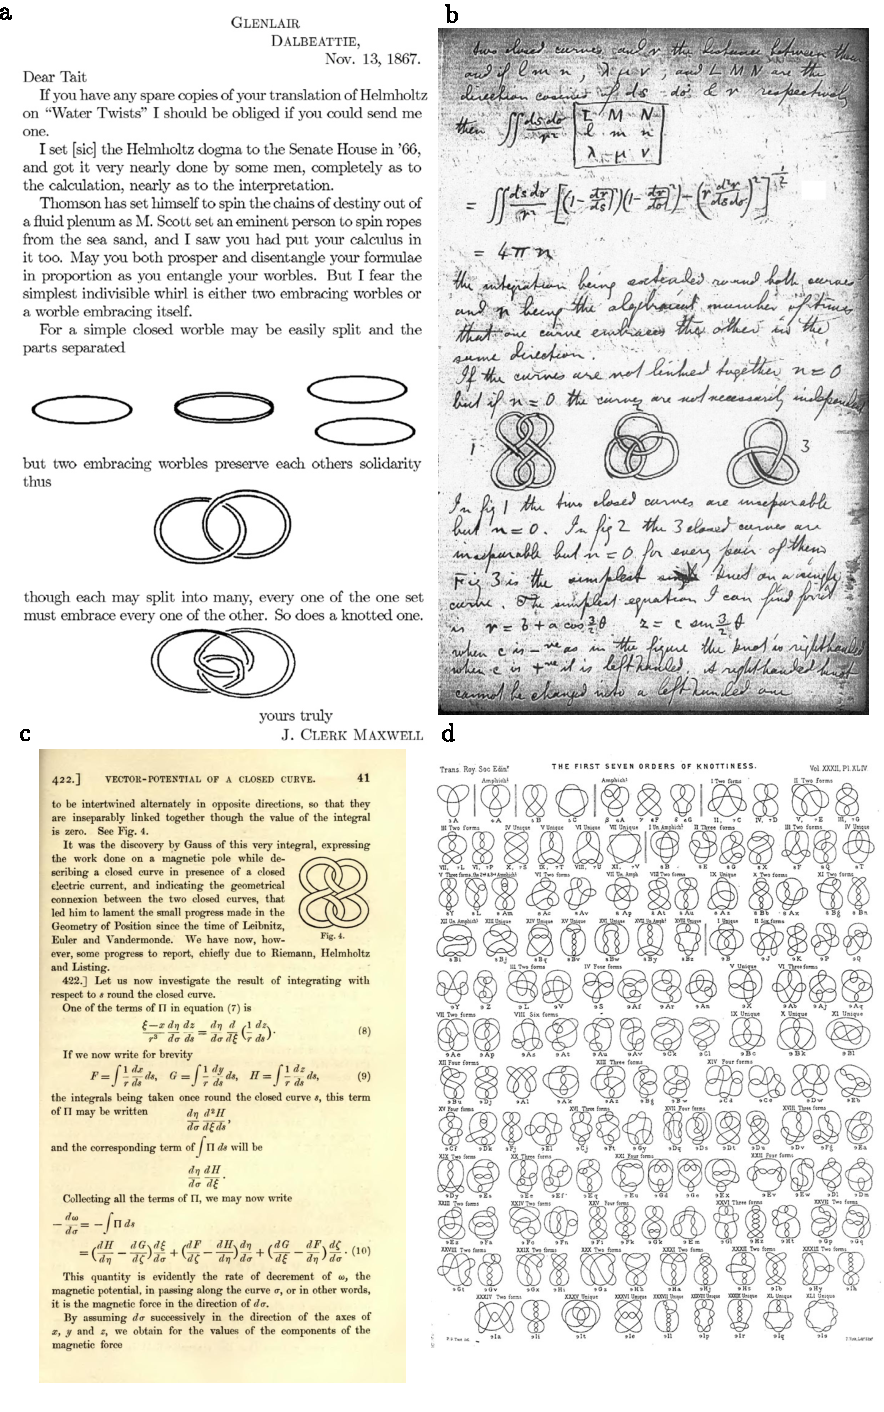
\includegraphics[width=0.9\linewidth]{\IntroductionFigures/History.pdf}
\caption{(a) 1867. Letter from Maxwell to Tait, encouraging him to ``prosper and disentangle your formulae in proportion as you entangle your worbles'' and requesting Tait's own translation of \citep{Helmholtz}. (b) 1867. Letter from Maxwell to Tait, showing a formula for Gauss's linking number alongside two links of linking number 0 and a trefoil knot. Reproduced from Ref.~\citep{Ricca2011}. (c) 1873. Page from Maxwell's \emph{A Treatise on Electricity and Magnetism}~\citep{Maxwell2}, giving a discussion of the Gauss linking number and the same example of linking number zero seen in (b). (e) 1876. The first iteration of Tait's knot tables \citep{Tait1}.}
\label{fig:History}
\end{figure}

Kelvin's ``vortex atom'' encountered difficulties in its mathematical content, its falsifiability, and a lack of contemporary experimental support \citep{KelvinMasters}. However its content, summarised as ``\textit{Physics = Geometry}'' in Ref.~\citep{KelvinAMS}, was compelling and apparently motivated Tait, in ``consideration of the forms of knots by Sir W. Thomson's (Lord Kelvin) Theory of Vortex Atoms'', to construct the first systematic tables of knots in 1876--1885, shown in figure \ref{fig:History} \citep{Tait1, Tait2, Tait3}. Tait's articles, alongside a ``very remarkable essay by Listing ... and an acute remark made by Gauss ... with some comments on it by Clerk-Maxwell''~\citep{Tait1} form the initial studies in what is now the mathematical field of knot theory \citep{Lickorish1997}. Maxwell himself, although not an active contributor to vortex atom theory, had a clear interest in the ideas, encouraging Tait in a letter in 1867 to ``prosper and disentangle your formulae in proportion as you entangle your worbles'' (figure \ref{fig:History}). Indeed the ``comments by Clerk-Maxwell'' referred to by Tait are in fact Maxwell's re-derivation of Gauss's linking number, as presented in his \textit{A Treatise on Electricity and Magnetism} \citep{Maxwell2} in 1873, about which we will have much more to say in \S\ref{ch:Maxwell}. 

Despite forming the starting point for modern knot theory, the knotted structures above are quite different to those found in your shoelaces, or in the world of art and design outside the physics department. Rather than a single knotted curve, we have a continuous fluid in whose structure the knot is encoded, and from which dynamical properties of the knot (its motion, stability, a spectrum of vibrational modes etc.) may be derived. More precisely, we have a concentrated tube of vorticity in the fluid, tied into the shape of a knot. Helmholtz's laws of vortex motion \citep{Helmholtz} show that, in a perfect (frictionless) fluid this tube of vorticity is `frozen in' to the fluid, unable to dissipate or cross itself. In an idealised vortex atom, the radius of this tube would tend to zero, with the vorticity contained inside becoming infinite, and we would have a singular linelike structure, tied into a knot and embedded into a continuous three dimensional medium. This structure is our first example of what is called a \emph{knotted field}. There is no strict definition of what constitutes of a knotted field, but a sensible operational one is that they are physical fields containing knotted, linked, or otherwise topologically interesting structure, and that this structure has some interplay with the behaviour of the whole field. As we shall see, such fields are certainly not confined to fluids.

The disconnect between a knotted curve and a knotted field is reflected in Tait's work, which mentions Kelvin's Vortex Atoms briefly as motivation, but focuses in substance on ``the investigation of the essentially different modes of joining points in a plane'' \citep{Tait1}. As knot theory developed, its initial connections to hydrodynamics and electromagnetism were further abandoned. One also notes that despite the wonderful knot tables produced by Tait (figure \ref{fig:History}) and the reliance of vortex atom theory on knotted and linked vortices, there is no mention above of any experimental evidence of vortices tied in nontrivial knots. 
\begin{figure}[htbp]
\centering
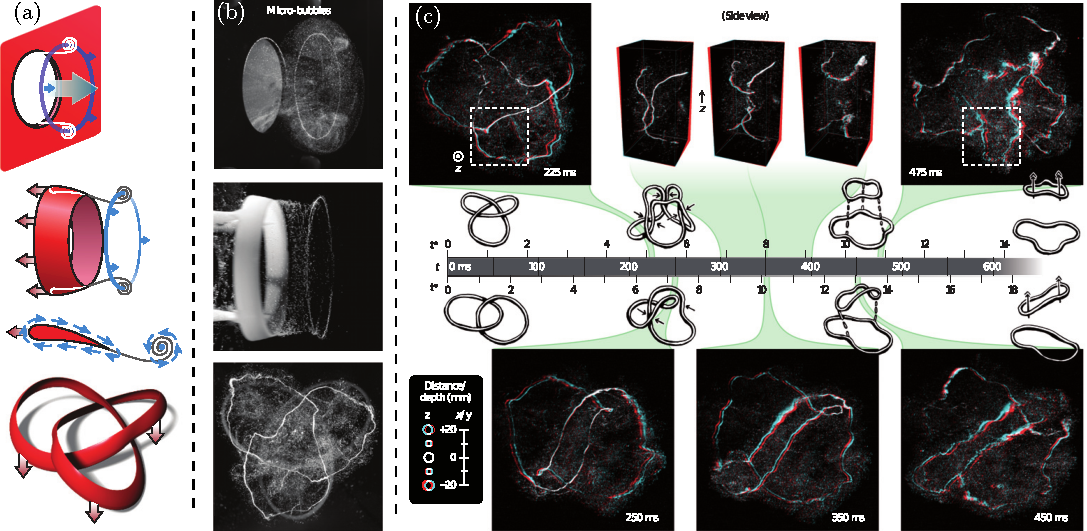
\includegraphics[width=1 \linewidth]{\IntroductionFigures/Irvine_Figs1_3.pdf}
\caption{The first experimental construction of fluid knotted vortices, in 2013. (a) Experimental methods for making knotted vortices. The hydrofoil (bottom three panels) is most successful. (b) Vortices produced in water from the designs of panel (a). Microbubbles track the vortex. The mean radius of the ring is $40$mm, of the trefoil $45$mm. (c) Timelines showing the evolution of a trefoil knot (top) and Hopf link (bottom) in three dimensions. In contrast to ideal fluids, we see progressive reconnections and simplification of the links. Figures reproduced from Ref.~\citep{Kleckner2013}.}
\label{fig:Irvine}
\end{figure}

The first experimental construction of nontrivial knotted fluid vortices came 146 years after their initial theoretical investigation, from the Irvine lab in 2013. We show in figure~\ref{fig:Irvine} several remarkable figures reproduced from Ref.~\citep{Kleckner2013}, in which Kleckner and Irvine tied a single vortex loop in water into a trefoil knot, the simplest nontrivial knot, as well as linking two vortex loops together (Kelvin's proposed model for a sodium atom), before tracking their full three-dimensional evolution. Ref.~\citep{Kleckner2013} is a notable example of a more general trend; over the past $\sim10$ years knotted fields have gone from being purely theoretical constructions to being experimentally realisable in a number of systems, and though originally conceived of in fluid dynamics, modern applications are not limited to this context; they have been realised as nodal lines of optical beams~\citep{Dennis2010}, as disclinations in nematic liquid crystals~\citep{Tkalec2011,Tasinkevych2014,Copar2015} and as spinor Bose-Einstein condensates~\citep{Hall2016}. In the following sections we will review the state of modern experiment and theory on knotted fields, beginning with fluids and superfluids, in some sense the most developed case, before moving on to parallel developments in liquid crystals and excitable media, which directly underlie the work presented in \S \ref{ch:FitzHughNagumo} and \S \ref{ch:TwistBend} in this thesis; these example are certainly not exhaustive, and focus on `soft matter' systems, a point we shall discuss at the end of the chapter. We shall see that the subject has broadened considerably since Kelvin's atoms and his contemporaries' study of fluids. There will be a commonality of ideas between the different disciplines mentioned above, but also genuine differences.
\section{Modern knotted fields: fluids}
\label{sec:Fluids}
With the decline of Kelvin's vortex atom theory and the development of knot theory away from its hydrodynamic origins, a resurgence of interest in knotted fields might be dated to the years 1958-1969, with Moreau and Moffatt's seminal papers on helicity in ideal fluids \citep{Moreau1961,Moffatt1969}, preceded by analogous results in magnetohydrodynamics by Woltjer \citep{Woltjer1958}. Focusing on the ideal fluid, both Moreau and Moffatt independently demonstrated that the helicity

\begin{equation}
    \mathcal{H} = \int {\bf u} \cdot {\boldsymbol{\omega}} \ d^3 \bf r,
\end{equation}
where ${\bf u}({\bf r},t)$ is the fluid velocity and $\boldsymbol{\omega} = \nabla \times \bf u$ is the vorticity \citep{Saffman1992}, is conserved under the Euler equations of ideal flow. Moffatt in particular gave this invariant a topological interpretation: it measures the linking of vortex tubes within the fluid. Given a fluid where $\boldsymbol{\omega}$ is concentrated along discrete sets of curves $C_i$, Moffatt showed that
\begin{equation}
    \mathcal{H} = \sum_{i,j}\Gamma_i \Gamma_j  Lk(C_i,C_j) 
\label{eq:OriginalHelicity}
\end{equation}
where $\Gamma_i$ is the vorticity flux along curve $C_i$, and $Lk(C_i,C_j), i\neq j$, is the Gauss linking number between curves $C_i, C_j$ (this interpretation of helicity actually extends to the case where the vorticity is not concentrated along a finite set of curves, but is distributed throughout the fluid \citep{Arnold1999}). The meaning of $Lk(C_i,C_i)$ will be clarified below. Figure~\ref{fig:Moffat} shows several examples of vortex tubes with different linking numbers and hence helicities. Seen in this light, the conservation of helicity is a direct consequence of Helmholtz's laws of vortex motion, and is equivalent to the statement that initially linked vortex tubes remain so; in some sense it is remarkable that the result was not known to Kelvin and Maxwell.
\begin{figure}[htbp]
\centering
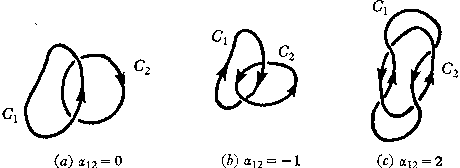
\includegraphics[width=1 \linewidth]{\IntroductionFigures/Moffat.pdf}
\caption{Three examples of links with different linking numbers. In the figure, $Lk(C_i,C_j)$ is denoted $\alpha_{ij}$. Figure reproduced from Ref.~\citep{Moffatt1969}.}
\label{fig:Moffat}
\end{figure}

When vorticity is not concentrated along a singular curve but distributed in a thin vortex tube, there is additional internal structure --- one imagines a ribbon (figure~\ref{fig:RibbonMontage}(a)), or braided rope (figure~\ref{fig:RibbonMontage}(b)). Flux lines may wind around the centre-line of this tube as in figure \ref{fig:RibbonMontage}(b), endowing it with a second linking number, the self-linking number, which measures the linking of any flux line with the curve centre-line. Incorporating this structure into the helicity count we find \citep{Moffat1992}
\begin{equation}
    \mathcal{H} = \sum_{i,j, i\neq j}\Gamma_i \Gamma_j  Lk(C_i,C_j) + \sum_{i} \Gamma_i^2 SL(C_i), 
    \label{eq:HelicityCount}
\end{equation}
where $SL(C_i)$ denotes the self-linking of each curve $C_i$ with its implicitly assumed ribbon. Defining $Lk(C_i,C_i) := SL(C_i)$ this expression reduces to~\eqref{eq:OriginalHelicity}. In Ref.~\citep{Moffatt1969} Moffatt does not explicitly consider a vortex tube, but nevertheless defines a `self winding number', which with the benefit of hindsight one interprets as the self-linking number of the simplest kind of tube, one made up of a family flux lines running parallel to one another. As we shall see below, that the flux lines are locally parallel does not imply $SL(C_i) = 0$.
\begin{figure}[htbp]
\centering
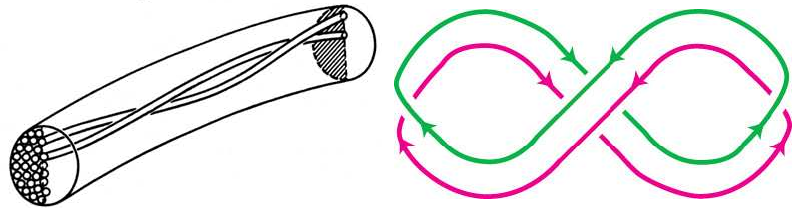
\includegraphics[width=\linewidth]{\IntroductionFigures/RibbonMontage.pdf}
\caption{A curve with internal structure: ribbons and tubes. (a) A ribbon, defined by a centre-line (pink, say) and a second offset curve (green). The diagram is a projection of the ribbon living in three dimensions, and each crossing may be annotated as either a twist $Tw$ or writhe $Wr$ crossing, depending on its local (green across pink, no pink across pink) or nonlocal (green across pink + pink across pink) nature. The total count gives a self-linking number for the ribbon; see~\eqref{eq:Count}. (b) A twisted tube, in which one particular `filament' may be arbitrarily chosen to define a ribbon. This is the situation in vortex tubes. Figures reproduced (modified) from Refs.~\citep{Dennis2005,Moffat1992}.}
\label{fig:RibbonMontage}
\end{figure}
\subsection{C\u{a}lug\u{a}reanu's theorem, real fluids}
Given a ribbon diagram like figure~\ref{fig:RibbonMontage}(a), the self-linking number may be further decomposed as
\begin{equation}
    SL = Tw + Wr.
    \label{eq:Count}
\end{equation}
The first term, the twist $Tw$, counts the local crossings of the ribbon over its centre-line. The second term, the writhe $Wr$, counts non-local crossings of the ribbon over distant parts of the centre-line. In figure~\ref{fig:RibbonMontage} each crossing of the ribbon over its centre-line is annotated with the nature of its contribution. Note that the $Wr$ count is actually independent of the choice of ribbon. For different diagrams of the same knotted ribbon each of these contributions varies, but their sum $SL$ does not. Averaging over also possible diagrams, i.e. all possible projections of the genuine three-dimensional curve, one obtains integral formulae for twist and writhe, and in this form the result~\eqref{eq:Count} was first discovered by Georges C\u{a}lug\u{a}reanu \citep{Calugareanu1959,Calugareanu1961} (the interpretation of it given above is however due to Ref.~\citep{Dennis2005}). C\u{a}lug\u{a}reanu's Theorem is an important and influential result, finding application in Mathematics~\citep{White1969,Adams2004,Aldinger1995}, Physics~\citep{Moffat1992, Goldstein1995, Berger2006}, Biology~\citep{Fuller1978, Winfree1983, Sumners1995} and beyond. It is of potential relevance whenever one studies the properties of a curve with some internal structure, and so it naturally appears frequently in the study of knotted fields. It will play a role in the curve dynamics studied in \S\ref{ch:FitzHughNagumo}, in conservation laws encountered in \S\ref{ch:TwistBend} and, in its close connection to Maxwell and Gauss's work on linking numbers and electromagnetism, in \S\ref{ch:Maxwell} as well. For the purposes of the current discussion it enables us to speak of writhe helicity $Wr$ and twist helicity $Tw$, two separate contributions to the total helicity count. All three modes of helicity storage are shown in figure~\ref{fig:Irvine2}(a). Assuming all vortices in the system have the same flux $\Gamma$ we have that
\begin{equation}
 \mathcal{H} = \Gamma^2\sum_i \sum_{j \neq i} Lk(C_i,C_j) + Tw(C_i) + Wr(C_i).\label{eq:twistpluswrithe} 
\end{equation}
To return again to Moffatt's original result \eqref{eq:OriginalHelicity}, a locally parallel bundle of tubes has $Tw(C_i) =0$, and only contains writhe helicity, as in the $Wr$ component of figure \ref{fig:Irvine2}(a) --- in other words here $SL(C_i) = Wr(C_i)$. In this case \eqref{eq:twistpluswrithe} reduces to \eqref{eq:OriginalHelicity}. Consistent with this fact, $Wr(C_i)$ may be computed from the curve $C_i$ only, without the need to explicity consider a tube at all (further, the integral formula for the Gauss linking number reduces to the integral formula for writhe when the curves involved coincide \citep{Moffat1992}), and so if one neglects internal tube structure they will pick up the $Wr$ but not the $Tw$ contributions to helicity; this is referred to as the centre-line helicity $\mathcal{H}_c := Lk +Wr$ \citep{Scheeler2014}.

In a real (viscous) fluid, helicity is not \emph{a priori} conserved. The question of whether it is in practice, and the mechanism of its dissipation, are areas of active research \citep{Kleckner2013, Scheeler2014,Scheeler2016}. Naively, one expects the reconnections shown in figure~\ref{fig:Irvine} to be accompanied by jumps in the value of helicity. Ref.~\citep{Scheeler2014} measured the centre-line helicity $\mathcal{H}_c$ across reconnections in trefoil knots and Hopf links, as shown in figure~\ref{fig:Irvine2}(b).They found that $\mathcal{H}_c$ is in fact not dissipated in a reconnection, but rather transferred from $Lk$ to $Wr$. Ref.~\citep{Scheeler2016} measured all three contributions to $\mathcal{H}$ including $Tw$ in a system of unlinked rings, finding $Tw$ to be dissipated by viscosity, but the remaining contribution $\mathcal{H}_c$ preserved (figure~\ref{fig:Irvine2}(c)). Taken together the results suggest that helicity is primarily dissipated on small scales via the $Tw$ term, and not by reconnections as might have been expected --- this leads to approximate conservation of helicity over surprisingly long timescales.
\begin{figure}[htbp]
\centering
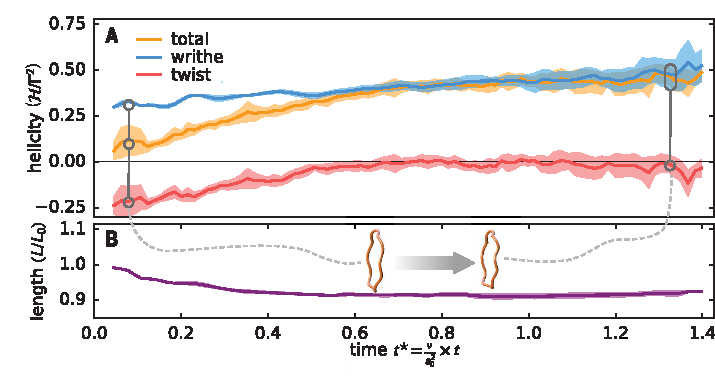
\includegraphics[width=0.9\linewidth]{\IntroductionFigures/Irvine2.pdf}
\caption{Evolution of helicity in a viscous fluid. (a) The three modes of helicity storage: linking $Lk$ of two vortex tubes, writhing $Wr$ of the centre-line of a single tube, and twisting $Tw$ of the vortex tube about the centre-line. (b) Experimental data (blue curves raw data, orange curves smoothed) tracking centre-line helicity $\mathcal{H}_c := Lk + Wr$ evolution for a trefoil knot and Hopf link, showing that $\mathcal{H}_c$ is conserved across reconnections. (c) The three contributions to helicity are experimentally tracked as a vortex ring evolves. Twist helicity $Tw$ dissipates to zero, but writhe helicity $Wr$ is conserved. (d) The experimental setup allowing the measurements shown in panel (c). Tangential flow resolution along the vortex core is enabled by impregnating an aerofoil with separated blobs of dye, which are traced over time. Figures reproduced from Refs.~\citep{Scheeler2014, Scheeler2016}. }
\label{fig:Irvine2}
\end{figure}

\subsection{Fluids as a case study}
The hydrodynamic (and magnetohydrodynamic) story of knotted fields is well developed. We have given a sketch, but the reader is invited to find more detail in reviews such as Refs. \citep{Moffatt2014, Irvine2018}. Outside of hydrodynamics the above discussion acts as a template for what one might expect in knotted fields more generally; a test case which other systems may be compared to and contrasted against. In particular, linking and self-linking of structure occur in a variety of contexts, and in analogy to~\eqref{eq:twistpluswrithe} one might seek to connect them to conserved quantities, and use them to understand the dynamics of the entire system under study. To give a brief example of a system for which this template is fruitful consider superfluids, close cousins of normal fluids described by a complex scalar field $\psi = |\psi| e^{i \phi}$ (figure~\ref{fig:SuperFluidMontage}(a)) evolving via the non-linear Schr\"odinger equation \citep{Kleckner2016}. Here vortices are given by singular lines where the circle-valued phase field $\phi$ is undefined, and about which it winds by $2\pi$. As in fluids, one may define a notion of helicity, initialise knotted vortices and study their evolution (figure~\ref{fig:SuperFluidMontage}(b)) \citep{Scheeler2014, Kleckner2016}. The definition of centre-line helicity $\mathcal{H}_c := Lk + Wr$ carries through, and its evolution turns out to be similar to that of viscous fluids \citep{Scheeler2014, Kleckner2016}; reconnections occur in similar manner, and they approximately preserve the centre-line helicity $\mathcal{H}_c$.\footnote{ \label{footnote:Seifert} Construction of the full helicity $\mathcal{H}$ is harder: the natural ribbon structure for a single superfluid vortex is given by its intersection with the surface $\phi =0$, the `Seifert framing'~\citep{Winfree1983c,MoffattBook} for which $\mathcal{H}=0$! See \citep{Salman2016,Salman2017,Kedia2018a} for a resolution to this apparent paradox. We will encounter Seifert framings again, canonically constructed by the solid angle function, in \S \ref{ch:Maxwell}.}
\begin{figure}[htbp]
\centering
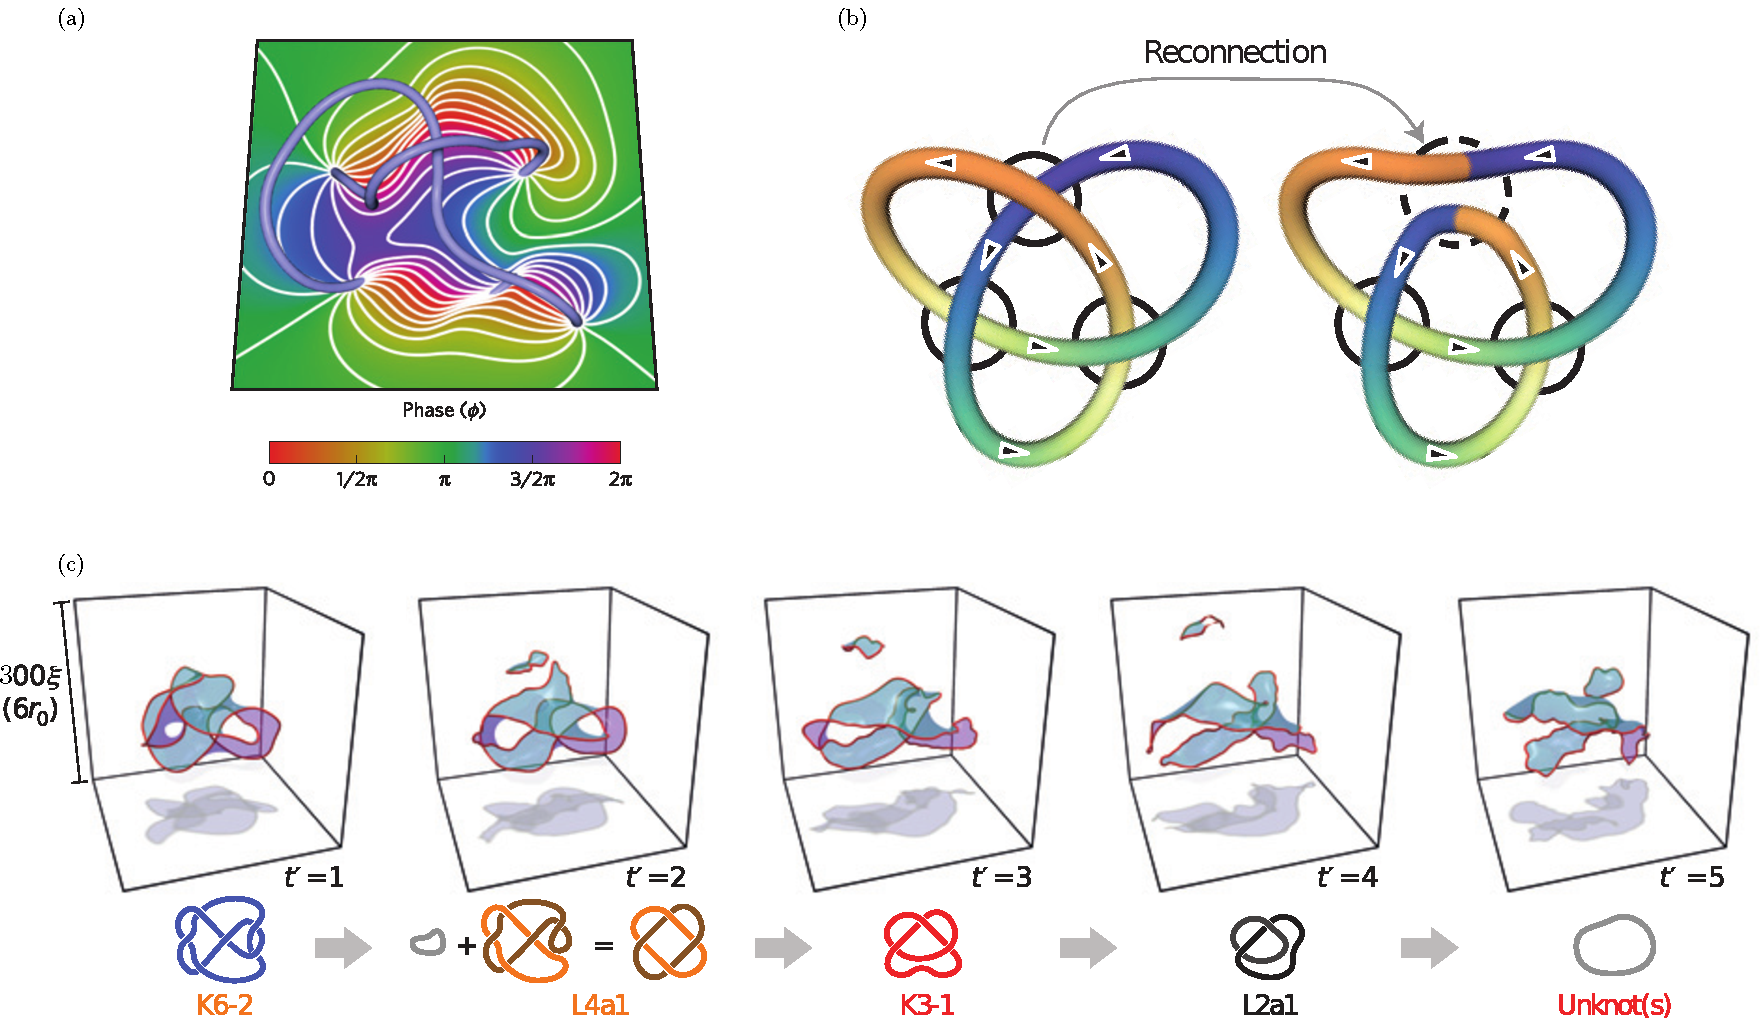
\includegraphics[width=\linewidth]{\IntroductionFigures/SuperFluidsMontage.pdf}
\caption{Evolution of superfluid vortex knots. (a) Cross section through a superfluid vortex knot (light blue curve), showing the phase field $\phi$ winding by $2 \pi$ about the vortex. (b) A schematic illustration of a reconnection. Colour is for visualisation only; note the splicing. (c) An example untying of a superfluid link into a collection of unknots by progressive reconnections. Blue surfaces spanning the knot are surfaces of constant phase. A schematic of the untying process is shown below.}
\label{fig:SuperFluidMontage}
\end{figure}

However, it is not the case that knotted fields in all other systems may be understood simply through the lens of fluids. In the following section we turn to the second experimental system with which substantial work on knotted fields has been done, the nematic liquid crystal cells of Refs.~\citep{Tkalec2011,Tasinkevych2014,Copar2015}. There will be some crossover with the discussion above, but also genuine differences, especially in the theoretical constructions involved. 
\section{Modern knotted fields: liquid crystals}
\begin{figure}[htbp]
\centering
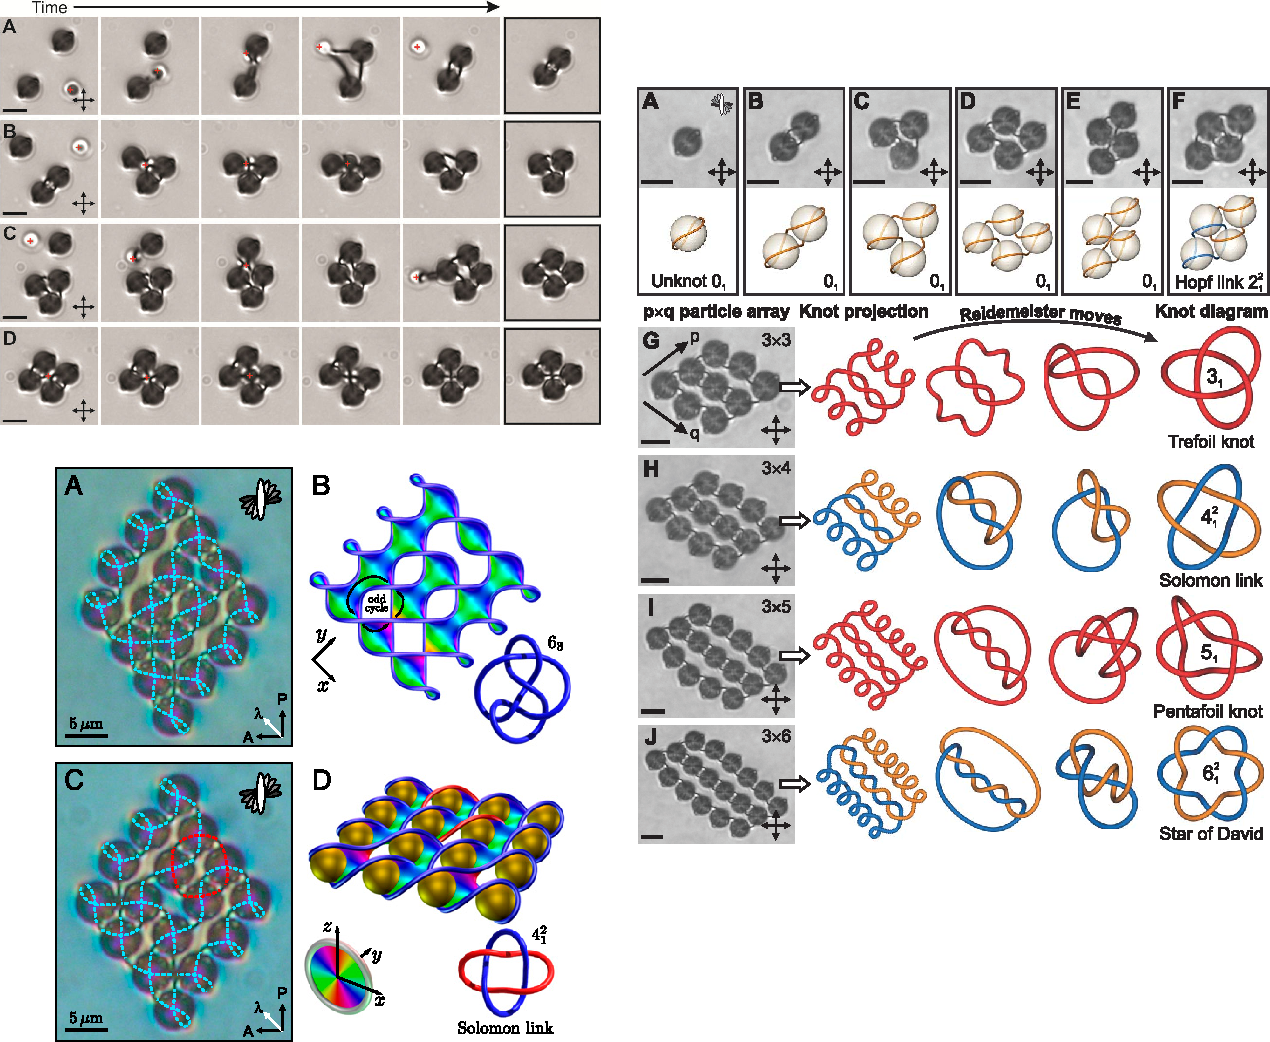
\includegraphics[width=0.8 \linewidth]{\IntroductionFigures/LiquidCrystalMontage.pdf}
\caption{Knotted disclination lines. (a) Nematic disclinations (dark curves) are wrapped around silica colloids 4.82 $\mu$m in diameter (dark spheres), initially in `Saturn's ring' configurations. Both disclinations and colloids may be manipulated by laser tweezers (red dot). The figure shows controlled assembly of an array of colloids with a single defect line wrapped about them. Black scale bar 5 $\mu$m. (b) Any knot or link may be constructed around these colloidal arrays. The figure shows the experimental assembly of a Hopf link alongside simulation predictions of its shape at each stage, as well as several other completed knots and links. (c) Within two finished links, the sense in which the director $\bf n$ is twisting is shown with colouring: the background dark blue corresponds to one handedness, with regions of light colour denoting its reversal. This visualisation allows construction of the Pontryagin-Thom (PT) surface for the link, which in turns allows homotopy classification~\eqref{eq:HomotopyClassification}. Figures reproduced from Refs.~\citep{Tkalec2011,Copar2015}.}
\label{fig:KnottedLiquidCrystal}
\end{figure}
A second experimentally constructed knotted field is shown in figure~\ref{fig:KnottedLiquidCrystal}. It is quite different to that of figure~\ref{fig:Irvine}. By including microscopic colloids a few $\mu$m wide into a thin cell of nematic liquid crystal, experimentalists~\citep{Tkalec2011,Tasinkevych2014,Copar2015} are able to force the appearance of defect lines in the material. These defects may then be manipulated with laser tweezers, and by weaving them about an array of colloids, a knotted field encoding any type of knot or link can be constructed; unlike the fluid vortices above, these structures are stable, able to be experimentally probed in some detail. This system provides a testbed for a series of new ideas about knotted fields, but first we step back a moment and provide a brief description of what liquid crystals, defects and colloids etc. actually are.

\subsection{A brief introduction to liquid crystals}

Liquid crystals are a class of materials which possess properties associated to both liquids and solids~\citep{deGennes1992}. In their most common form, the nematic phase, they show no positional order, and flow like a liquid. However, they do show orientational order: if one attempts to twist a portion of the liquid crystal it will respond elastically, as a solid would\footnote{This is remarkable: imagine your surprise if, upon attempting to stir your coffee, you found it fiercely resisted your attempts to turn the spoon, but was nevertheless happy to be poured down the sink.}. The microscopic basis for this behaviour comes from the type of molecules which comprise nematics, two examples of which are shown in figure~\ref{fig:DeGennesMontage}(a)--(b); they are typically thin rods which locally align themselves along some common axis without taking on any sort of crystalline positional order. In continuum theories this orientational order is described by a spatially varying unit vector field $\bf n$, called the director, which represents an average local molecular orientation, as shown in figure~\ref{fig:DeGennesMontage}(c).
\begin{figure}[htbp]
\centering
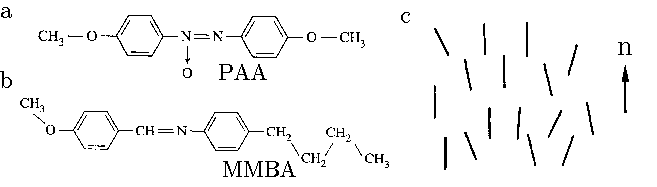
\includegraphics[width=1\linewidth]{\IntroductionFigures/DeGennesMontage.pdf}
\caption{(a,b) Two example of molecules which can form a nematic liquid crystalline phase. (a) p-azoxyanisole (PAA) forms a nematic between $116$--$135^\circ$C at atmospheric pressure. (b) N-p-methoxybenzylidene-p-butylanilinie (MMBA) forms a nematic between $20$--$47^\circ$C. (c) A schematic of local molecular alignment, with the director $\bf n$ giving a direction averaged over microscopic lengthscales. Figures reproduced (modified) from Ref.~\citep{deGennes1992}}
\label{fig:DeGennesMontage}
\end{figure}

The theory of their elastic distortions contains much interesting geometry which we will return to in \S \ref{subsec:Geometry}, but for an understanding of figure~\ref{fig:KnottedLiquidCrystal} we instead focus on a celebrated feature of nematics \citep{Frank1958}, their topological defects. If one shines polarised light through a thin slice of nematic placed between crossed polarisers, they will observe something like figure~\ref{fig:Disclination}~(a), a schlieren texture\footnote{The word `texture' is commonly used to describe liquid crystal configurations more generally.} \citep{deGennes1992}. Places in the sample where the director $\bf n$ is aligned with one of the two polariser directions H and V do not transmit light, leading to the dark brushes observed. One immediately notes points where the brushes meet, sometimes with two brushes leading into a point, sometimes four; a point of each type is marked in figure~\ref{fig:Disclination}(a). What is the structure of the director at these points? The confluence of dark brushes implies that, in a small circle around these points, the director winds, and that at the point itself we cannot consistently define $\bf n$; these points are topological defects, places where the order breaks down. Traversing such a circle around a point with two brushes, the director is aligned with each of H and V only once; in other words it makes only half a turn in a full circle around the defect. This observation is enough to establish that the director $\bf{n}$ must in fact be non-orientable; it should not be thought of as a vector field, but as a line field, for which $\bf n \sim - \bf n$.
\begin{figure}[htbp]
\centering
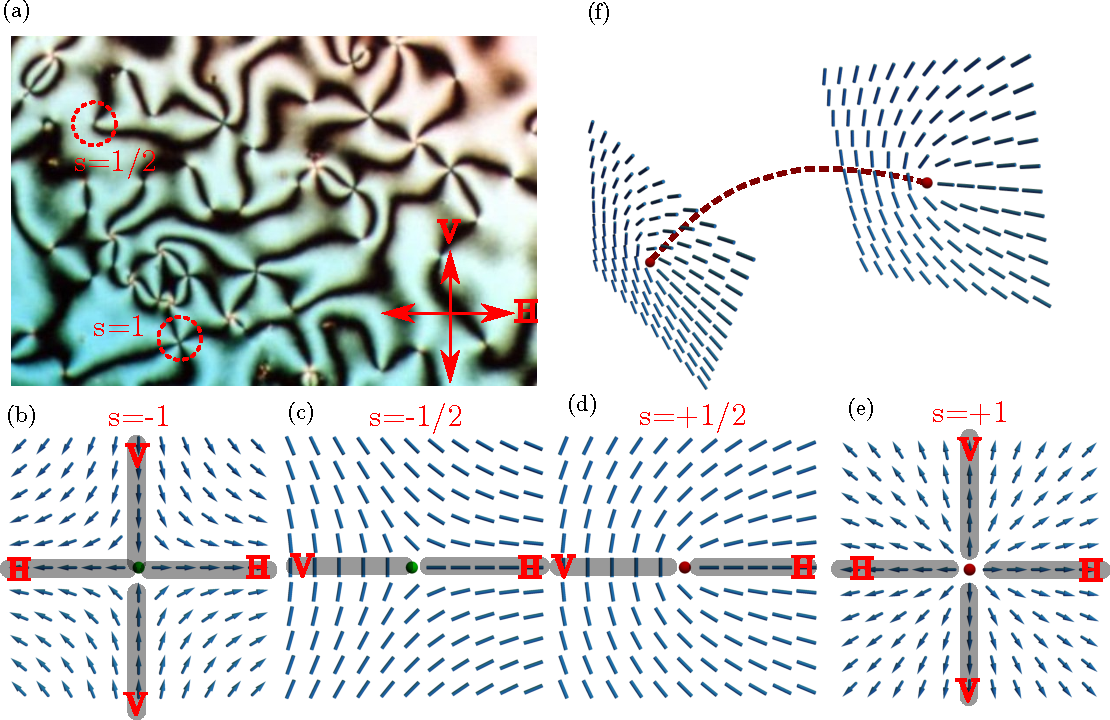
\includegraphics[width=1\linewidth]{\IntroductionFigures/DisclinationLine.pdf}
\caption{Topological defects in liquid crystals. (a) A schlieren texture, with crossed polariser directions overlaid, and defects of winding number (denoted s) $\frac{1}{2}$ and $1$ highlighted (one cannot distinguish $\pm$ from the picture alone). (b)--(e) Topologically accurate director configurations around defects of winding number $\pm \frac{1}{2}$, $\pm1$, with the schlieren dark brushes overlaid. For $\pm1$ defects it is possible to orient the director, and we have made one of the two possible choices of arrowheads. (f) Schematic of a disclination line in a three-dimensional nematic sample, with two cross sections showing local structure. Locally, there is only one type of disclination line ($\pi_1(\mathbb{R}P^2) \approx \mathbb{Z}_2$) so a winding is not given.}
\label{fig:Disclination}
\end{figure}
In figures~\ref{fig:Disclination}(b)--(e) we show qualitative configurations of the director around these defects, with their associated schlieren texture brushes. In figures~\ref{fig:Disclination}(b),(e) we have four brushes, and a line field which can be oriented; to emphasise this fact we have decorated the line field with one of the two possible choices of arrowheads. Figures~\ref{fig:Disclination}(c),(d) correspond to the non-orientable two brush case; here one cannot consistently assign arrowheads to the rods (it is worth trying to imagine doing so). Note that from a single image such as figure~\ref{fig:Disclination}(a), we cannot distinguish defects winding in a right handed sense ($+\frac{1}{2}, +1$ etc. in the figure) from left handed by counting brushes. In two dimensions these defects, also called disclinations or dis\emph{in}clinations \citep{Frank1958}, are points, but in three dimensions they are lines, transverse cross sections of which have local profiles resembling the two dimensional case; a schematic illustration is shown in figure~\ref{fig:Disclination}(f). As with fluid vortices, these disclination lines may be knotted and linked together, and the variation of the local profile along the disclination (see the cross sections in figure~\ref{fig:Disclination}(f)) provides internal structure giving rise to self-linking~\citep{Copar2011}.

\subsubsection{Experiments on knotted disclination lines}

We now return to the experiments of Refs.~\citep{Tkalec2011,Tasinkevych2014,Copar2015}. In contrast to the situation in fluids, one of the major advantages of working with liquid crystal disclinations is the control experimentalists have over them. By including microscopic silica spherical colloids (4.72 $\mu$m diameter in figure~\ref{fig:KnottedLiquidCrystal}) into a sample of liquid crystal with specific surface anchoring conditions, experimentalists may frustrate alignment of the director $\bf n$ in a controlled fashion, necessitating the appearance of disclination lines. For example, in a thin cell of liquid crystal treated to promote uniform alignment of $\bf n$ within the sample, the inclusion of a colloid with normal anchoring conditions forces the appearance of a defect line around it to cancel the colloid's topological charge (it effectively acts as a point defect) and allow $\bf n$ to relax to uniform at large distances. Two such ``Saturn's ring'' configurations may be seen in the first frame of figure~\ref{fig:KnottedLiquidCrystal}(a). Once generated, these disclinations, as well as the colloids they wrap around, may be further manipulated using laser tweezers \citep{Tkalec2011}, as shown in the remainder of figure~\ref{fig:KnottedLiquidCrystal}(a). When two of these colloids are brought together the disclinations, either spontaneously or induced by the tweezers, fuse together (figure~\ref{fig:KnottedLiquidCrystal}(a), top row). Assembling an array of these colloids and weaving the disclination lines around them, the setup of Refs.~\citep{Tkalec2011,Tasinkevych2014,Copar2015} allows targeted construction of any knot or link; examples of some possible link topologies are shown in figure~\ref{fig:KnottedLiquidCrystal}(b). This system strikingly illustrates that knotted fields have more structure than a single knotted curve --- the curve organises the entire field (in this case the director $\bf n$) around it. Figure~\ref{fig:KnottedLiquidCrystal}(c) shows the knotted liquid crystal coloured by whether the director is twisting in a right or left handed sense. We see that the disclinations separate the liquid crystal into alternately right and left handed regions. In fact this division allows construction of a surface spanning the disclinations called the Pontryagin-Thom (PT) surface \citep{ChenThesis,Chen2013}, shown as the coloured surfaces in figure~\ref{fig:KnottedLiquidCrystal}(c), which classifies the topology of this liquid crystal texture; we shall return to this surface in a moment.

Let us compare the phenomena seen here to those in \S\ref{sec:Fluids}. In contrast to fluid vortices, it is experimentally possible to stabilise liquid crystal disclinations with colloids. This fact alone leads to many differences in the character of theoretical work on them. In the absence of the stabilising colloids the disclinations will shrink under effective line tension and undergo reconnections, however there is relatively little theoretical work on possible conservation laws analogous to~\eqref{eq:HelicityCount} or on the structure of these reconnections, although some results do exist \citep{Copar2011,Machon2017}. In this sense the dynamics of these knotted fields is less understood than is the case in fluids. It turns out, however, that there is much to be understood even about the statics of knotted liquid crystal fields. In a slice of liquid crystal we saw there were many types types of defect, indexed by the winding of the director --- what of liquid crystal textures in three dimensions? More specifically, given the knotted disclinations shown in figure~\ref{fig:KnottedLiquidCrystal}, are the liquid crystal textures corresponding to them unique, or are there many inequivalent possibilities? Questions like these have a long history in liquid crystal physics which, coupled with the difference in experimental possibilities we saw above, makes some split between the character of work on knotted fields in fluids and that in liquid crystals expected.

\subsection{Homotopy theory of knotted disclinations and Pontryagin-Thom surfaces}
\label{subsec:HomotopyTheory}
The traditional method of understanding liquid crystal textures containing defects is to place a measuring surface around a defect and study the possible textures on this surface, i.e. the different classes of map from the measuring surface to the space of possible values the order takes. Maps are equivalent when a continuous deformation, called a homotopy, exists between them, and as such this framework is known as the homotopy theory of defects \citep{Mermin1979,Alexander2012}. For point defects in a two-dimensional slice of nematic, this is what we did above, using a circle as our measuring surface. There, the space of possible directions $\bf n$ can point in is $S^1/\{x\sim-x\}$, the circle with antipodal points identified, also called the real projective line $\mathbb{R}P^1$. Thus the different classes of texture are reduced to the classification of maps ${\bf n}:S^1 \rightarrow \mathbb{R}P^1$ up to homotopy. This set of homotopy equivalence classes is denoted $[S^1,\mathbb{R}P^1]$. Actually computing this set is the work of algebraic topology \citep{Hatcher2012}, in which the set of homotopy classes of maps from a sphere $S^n$ into a space $X$, $[S^n,X]$, may be given a group structure after fixing a point $\star \in X$ and is called the homotopy group $\pi_n(X)$. It is found that $\pi_1(\mathbb{R}P^1) \approx \mathbb{Z}$ and thus there are infinitely many types of point defect in two dimensions as far as the traditional form of the theory is concerned; we show the four simplest in figure~\ref{fig:Disclination} but the index extends infinitely in both $+$ and $-$ senses. In three dimensions, the director takes values in $S^2/\{x\sim-x\}$, the sphere with antipodal points identified, also called the real projective plane $\mathbb{R}P^2$. Encircling a disclination line with a measuring loop as shown in figure~\ref{fig:RP2}, one finds $\pi_1(\mathbb{R}P^2) \approx \mathbb{Z}_2$, and thus there is exactly one type of disclination line, corresponding to the single nontrivial element of $\mathbb{Z}_2$\footnote{ One understands this difference by allowing the director in figure~\ref{fig:Disclination}(b,e) to buckle out of the plane of the paper, reducing these textures to the trivial one. This ``escape in the third dimension'' causes $\mathbb{Z}$ to undergo a mod 2 reduction.}.
\begin{figure}[htbp]
\centering
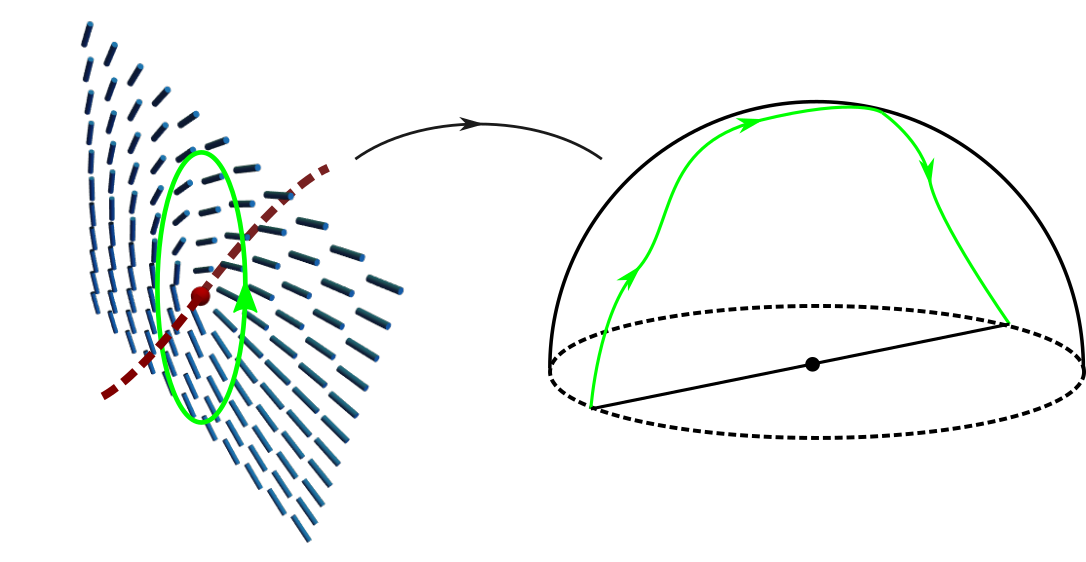
\includegraphics[width=0.9\linewidth]{\IntroductionFigures/RP2.png}
\caption{Application of the homotopy theory of defects to disclination lines. We place a measuring loop (green) around a disclination line (red curve). We then regard the director $\bf n$ (blue cylinders) as a map from this loop to the order space of the director, in this case $\mathbb{R}P^2$, modelled here as a hemisphere with equatorial points identified (pairs of red, blue, green dots indicate this identification). Homotopy theory then classifies this map as an element of $\pi_1(\mathbb{R}P^2) \approx \mathbb{Z}_2$. In this case the green curve on $\mathbb{R}P^2$ gives the single nontrivial element. If our measuring loop misses the disclination (purple) it traces a trivial path in $\mathbb{R}P^2$.}
\label{fig:RP2}
\end{figure}

A limitation of this approach is that, in only considering the texture on a specific measuring surface (in practice a sphere of some dimension) it discards information about the rest of the texture, which leads to ambiguities when considering multiple defects or more complex structures such as knotted and linked disclinations \citep{Alexander2012,Machon2014,Machon2016,MachonThesis}. A more recent, global approach \citep{Machon2014,Machon2016,MachonThesis} does not fix a measuring surface, but instead classifies maps into $\mathbb{R}P^2$ where the domain is the entire liquid crystal sample $M$ minus some set of (possibly knotted and linked) disclination lines $L$. The result is that the set of homotopy classes of the director is given by
\begin{equation}
[M-L, \mathbb{R}P^2] \approx H_1(\Sigma(L); \mathbb{Z})/\{ x \sim -x\},
\label{eq:HomotopyClassification}
\end{equation}
where $\Sigma(L)$ is the branched double cover of the link complement (its appearance in the result is a consequence of director non-orientability), and $H_1(\Sigma(L); \mathbb{Z})$ is its first homology group\footnote{An aside: if the order space is $ \mathbb{R}P^1 \approx S^1$, i.e. if one considers a phase field or a nematic confined to lie in a plane, then $[M-L, S^1] \approx H_1(M-L) \approx \mathbb{Z}$ \citep{Lickorish1997}. Such vortex lines are simply classified by their winding number, with no more internal structure.}. Without going into the details of this result, it is clear that these homotopy classes are far richer than the traditional classification scheme for disclinations would suggest, and that they depend strongly on the knot or link under consideration. To illustrate this point, in figure~\ref{fig:MachonMontage} we reproduce a `periodic table' of possible textures for $(p,q$) torus links from Ref.~\citep{MachonThesis}. Taking the simplest example from this table we see that for the Hopf link, consisting of two curves passing through each other once and given by $(p,q)=(2,2)$, there are exactly two nonhomotopic textures. Returning to the knots shown in figure~\ref{fig:KnottedLiquidCrystal}, for each knot there may be many nonhomotopic textures, and the knot diagram alone does not tell us which has actually been made. How should we extract this information, and visualise distinct textures? In figure~\ref{fig:Disclination} simple pictures of the director in the vicinity of a defect prove informative, but the same cannot be said of a swarm of sticks in three dimensions.
\begin{figure}[htbp]
\centering
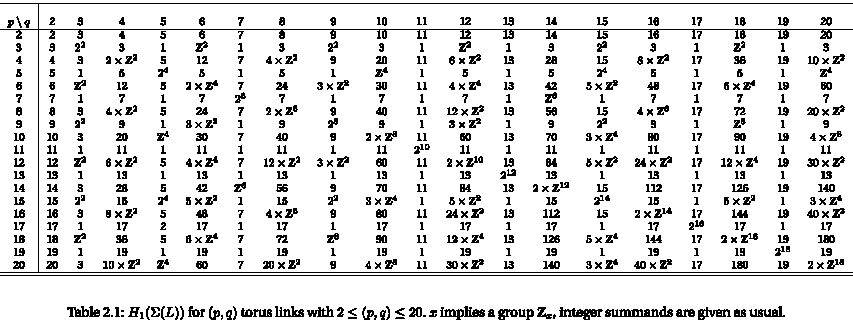
\includegraphics[width=\linewidth]{\IntroductionFigures/MachonMontage.pdf}
\caption{A `periodic table' of homotopy classes of nematic textures for $(p,q)$ torus links. Note the diversity: the sets may be finite or infinite, the number of $\mathbb{Z}$ components varies, and the number of elements in the finite component of each set may vary dramatically.}
\label{fig:MachonMontage}
\end{figure}

One solution is a construction which generalises the dark brushes of schlieren textures to three dimensions --- the Pontryagin-Thom construction \citep{ChenThesis,Chen2013,MachonThesis,AlexanderBook}. The idea is to extract the set of all points in the liquid crystal domain where the director lies in the  horizontal plane --- more precisely, perpendicular to some fixed direction in $\mathbb{R}P^2$ which we call the vertical axis. This is exactly what a schlieren textures shows in a two dimensional slice using $\mathbb{R}P^1$ instead, although schlieren textures contain some redundancy, showing us the set where the director is along some direction ($V$ in figure~\ref{fig:Disclination}(a), say) and also perpendicular to that direction ($H$ in figure~\ref{fig:Disclination}(a), the analogy to the horizontal plane in a three-dimensional texture)  --- we only really need half this data. In a three dimensional sample this `horizontal set' is not comprised of lines as in the two-dimensional schlieren texture but is a surface, the Pontryagin-Thom (PT) surface. After finding this surface, the construction is completed by colouring it according to the orientation in the horizontal plane that the director takes. An illustration of this procedure is shown in figure~\ref{fig:PT}(a). A powerful result in Algebraic Topology called the Pontryagin-Thom correspondence \citep{Milnor1997,Hatcher2012} shows that these coloured surfaces, taken up to smooth deformations (more precisely framed cobordisms), are in one-to-one correspondence with homotopy classes of maps, and so textures may be visually distinguished by their differing PT surfaces. To illustrate this fact, in figure~\ref{fig:PT}(b) we show the two distinct PT surfaces for the two nonhomotopic Hopf link textures~\citep{MachonThesis} (that they are both a single colour is an indication that representatives from both homotopy classes can be chosen with the director everywhere in the domain perpendicular to some axis, in particular one of the two horizontal axes). Returning to figure~\ref{fig:KnottedLiquidCrystal}(c), this construction provides the coloured surfaces shown; by examining the surface and the colour windings upon it, we may place the texture in one of the classes from~\eqref{eq:HomotopyClassification}. PT surfaces represent an enormous compression of information into a visually immediate form, and their utility is far from limited to disclination lines; we shall use them in our own work in \S\ref{ch:TwistBend}.

Now that we have seen some of the theoretical developments in knotted liquid crystals --- the homotopy classification, the Pontryagin-Thom construction --- let us remark again on the similarities and differences to fluids. Topological invariants play a vital role in both, linking and self-linking in fluids and homology groups of the link complement in liquid crystals. Indeed, the self-linking of liquid crystal textures will give rise to inequivalent colour windings on their PT surface and differing elements of the homotopy classification. However in contrast to fluids, where knot reconnections have been experimentally tracked and studied, there has been almost no mention of dynamics and link reconnections. When this happens, the topology of the link complement changes, and point defects may even be nucleated, perhaps a daunting theoretical task given that existing theory primarily assumes the domain is fixed, and even then finds a richness of possibility. We shall not develop this line of questioning further here, but invite the reader to consult Ref.~\citep{Machon2017} for theoretical developments in this direction. In summary, we simply remark that it is increasingly clear the world of knotted fields is far broader than fluids.

\begin{figure}[htbp]
\centering
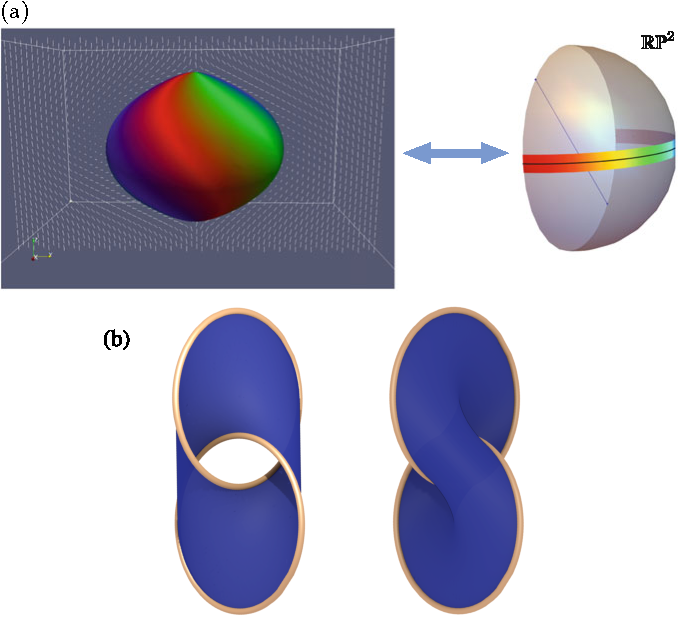
\includegraphics[width=0.8\linewidth]{\IntroductionFigures/PontryaginThom.pdf}
\caption{(a) The Pontryagin-Thom construction. The set where the director is horizontal is extracted and coloured by the angle the director makes in the horizontal plane (coloured band on $\mathbb{R}P^2$ with corresponding colours in the domain). Note that in contrast to the more standard picture of $\mathbb{R}P^2$ shown in figure~\ref{fig:Disclination} here it is `turned on its side' so that, visually, the horizontal plane through it (which one should imagine as also being the horizontal plane in the liquid crystal domain), does not coincide with the boundary of the hemisphere. The texture shown here is a topologically nontrivial one called a toron \citep{Smalyukh2010}, containing two strength $1$ point defects at its top and bottom, each detected by two rotations of the colour wheel on the PT surface. (b) Two distinct (noncobordant) PT surfaces for the Hopf link, representing the two possible nonhomotopic textures of figure~\ref{fig:MachonMontage}. Figures reproduced from Ref.~\citep{AlexanderBook,MachonThesis}.}
\label{fig:PT}
\end{figure}
\subsection{Beyond disclination lines}
The above sections focused on the knotting and nontrivial topology of disclination lines --- defects in the director $\bf n$ itself. Given the experimental focus on systems of this kind, and their direct connection to the idea of a knotted field, this is natural. However even in the absence of defects liquid crystals support an array of topological phenomena which may also be considered examples of knotted fields, although perhaps in a different sense to those discussed above. 

\subsubsection{Skyrmions and Hopfions}
\label{subsec:SkyrmionsAndHopfions}
The most well known topological feature of this kind is a Skyrmion, an example of which is shown in figure~\ref{fig:HopfionMontage}(a) given by the vector field ${\bf n}(r) = \cos(\pi r) {\bf e}_z + \sin(\pi r) {\bf e}_r$ on the unit disk. Fixing the director on the disk boundary, we may wrap this texture around a sphere (compactifying the boundary to a point) at which point its topology is captured by a map ${\bf n} : S^2 \rightarrow S^2$, in other words an element of $\pi_2 (S^2)\approx \mathbb{Z}$. These textures are a well studied feature of vector and line fields in two dimensions \citep{AlexanderBook}. We are primarily interested in the properties of order in three dimensions, and as such focus on their three dimensional `cousins': Hopfions.
\begin{figure}[htbp]
\centering
\includegraphics[width=0.8\linewidth]{\IntroductionFigures/HopfionMontage.pdf}
\caption{Defect free, topologically nontrivial textures. (a) A Skyrmion given by ${\bf n}(r) = \cos(\pi r) {\bf e}_z + \sin(\pi r) {\bf e}_r$, classified by an element of $\pi_2(S^2)\approx \mathbb{Z}$, here $+1$. One way to visualise this is by plotting the PT surface for the Skyrmion and noting its +1 winding. (b) An experimental image of a Hopfion in nematic order, with reconstructed PT surface. It is classified by an element of $\pi_3(\mathbb{R}P^2)\approx \mathbb{Z}$, here $+1$, which may be computed via the linking number of the different stripes of colour. That each colour occurs twice reflects that fact that the order space is $\mathbb{R}P^2$ not $S^2$ (see the following panels). (c,d) A simulation of of Hopfion in vector order (order space $S^2$), with stripes of two colours picked out to aid visualisation of their linking. Note that in vector order each colour only occurs once. (d) shows a cross section of the director field corresponding to this Hopfion. (e) Recent experimental image of a Hopfion, clearly showing the telltale linking of preimages. The first panel shows a vectorised director, i.e. a choice of arrowhead has been made. In the second panel, it has not, and linking of two colours for antipodal vectors becomes linking of the same colour. (f) Polarising optical micrograph of Hopfions and other textures. Arrows showed crossed polariser directions, and the green circled cross denotes the size of the laser tweezer which manipulates them. Panels (b,e,f) reproduced from Ref.~\citep{Chen2013,Ackerman2017}.}
\label{fig:HopfionMontage}
\end{figure}
An experimental image of a Hopfion is shown in figure~\ref{fig:HopfionMontage}(b)\citep{ChenThesis,Chen2013}. The figure shows a nematic liquid crystal texture inside a three dimensional cell, where the PT surface has been constructed by extracting director orientation via three-photon fluorescence microscopy. What qualifies the Hopfion as a knotted field becomes clear on viewing this surface: each stripe of colour twists about a torus, linking each other colour exactly once --- in a Hopf link, no less. Skyrmions are classified by an element of $\pi_2(S^2)$. Hopfions are instead classified by $\pi_3(S^2)$, the third homotopy group of the sphere. Heinz Hopf famously showed that $\pi_3(S^2) \approx \mathbb{Z}$, and in doing so constructed an explicit example of a nontrivial element of this group --- the celebrated Hopf fibration. For mathematical detail on the construction of the fibration we refer to the reader to Refs. \citep{BottTuBook,AlexanderBook}, and for an excellent video of its structure we urge the reader to consult Ref.~\citep{Johnson2011}. What figure~\ref{fig:HopfionMontage}(b) shows is an experimental image of this fibration; the energetics of the liquid system favour a fixed far field nematic direction, mimicking the Skyrmion boundary conditions and allowing the domain to be compactified  from $\mathbb{R}^3$ to $\mathbb{R}^3 \cup \textrm{pt} \approx {S}^3$. The nematic texture then realises a map ${\bf n}: S^3 \rightarrow \mathbb{R}P^2$, and $\pi_3(\mathbb{R}P^2) \approx \pi_3(S^2) \approx \mathbb{Z}$. The fact that the order lies in $\mathbb{R}P^2$ not $S^2$ is reflected in that fact that the fibration cycles through the colour wheel twice~\citep{Chen2013,Ackerman2017}; in figures~\ref{fig:HopfionMontage}(c)--(d) we show a Hopfion in vector order, in which each colour is only seen once. Two particular colours are picked out to make the linking clear.
\subsubsection{The geometry of vector fields}
\label{subsec:Geometry}
The linking of inverse images is the hallmark of the Hopf texture (figure~\ref{fig:HopfionMontage}(e)). However without data processing this linking is not an immediately apparent feature of the director. By contrast the knotted disclinations, and even their associated PT surface, in figure~\ref{fig:KnottedLiquidCrystal} may be clearly visualised. This is a consequence of the coupling of these topological features to the geometry, energetics and ultimately interaction with light of the liquid crystal, a coupling not present in the inverse images characterising the Hopfion in figure~\ref{fig:HopfionMontage}(e). This observation invites the question: are there `natural' features of the Hopfion, or nonsingular nematic-like liquid crystal textures in general, which can be used to infer their topology? We will explore this question, with a particular focus on the recently discovered twist-bend nematic phase~\citep{Lavrentovich2018}, in \S\ref{ch:TwistBend}. The focus will be on naturally geometric structures inside the liquid crystal which also contain some topological information, and so we now discuss the geometry of nematic-like liquid crystals, and vector fields more generally. 
\begin{figure}[htbp]
\centering
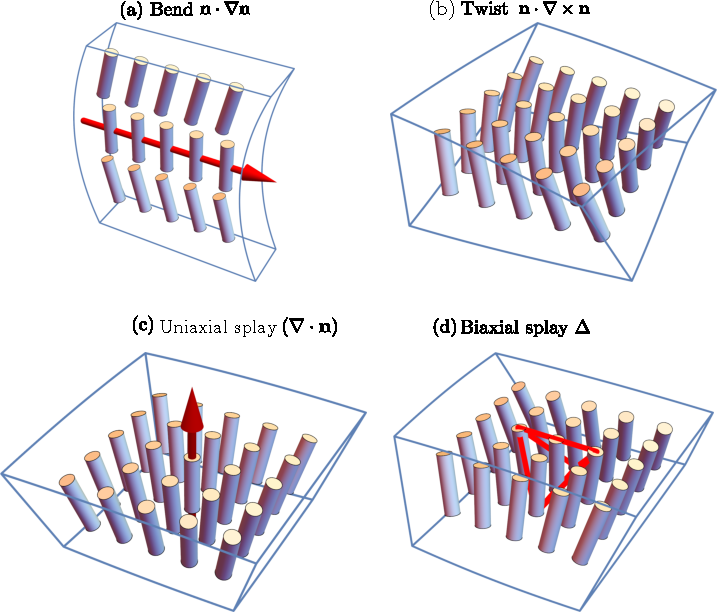
\includegraphics[width=0.7 \linewidth]{\IntroductionFigures/FrankFreeEnergy.pdf}
\caption{The four modes of director deformation: Bend, twist, (uniaxial) splay and biaxial splay. The vector plotted in (c) is the splay vector $(\nabla \cdot {\bf n}) \bf n$. Biaxial deformations, described by a rank two tensor (not a vector as in (a),(c)) are represented by a tetrahedron corresponding to the triple $\{{\bf n},\Delta_1, \Delta_2\}$, where $\Delta_i$ denotes the $i$th eigenvector of $\Delta$. Figures reproduced from Ref.~\citep{Selinger2019}. }
\label{fig:FrankFreeEnergy}
\end{figure}

The fundamental geometry and energetics of nematics was encoded by Frank in 1958~\citep{Frank1958}, where he gave a curvature free energy for their elastic distortions. We give this free energy here in a slightly nonstandard form, following Refs.~\citep{MachonThesis, Selinger2019}:
\begin{equation}
F = \int d^3 {\bf r} \quad \frac{K_1}{2} (\nabla \cdot {\bf n})^2 +\frac{K_2}{2} ({\bf n} \cdot \nabla \times {\bf n})^2 +\frac{K_3}{2}(({\bf n} \cdot \nabla) {\bf n})^2 - \frac{K_{4}}{2} \mathrm{det}(\Delta),
\label{eq:FrankFreeEnergy}
\end{equation}
where the various $K_i$ are elastic constants\footnote{These constants do not match one-to-one with those found in the standard writing of the Frank free energy; see Ref.~\citep{Selinger2019}.}. Each term in~\eqref{eq:FrankFreeEnergy} comes from a different mode of distortion for the liquid crystal, shown in figure~\ref{fig:FrankFreeEnergy}:
\begin{eqnarray}
    &({\bf n} \cdot \nabla) {\bf n} \quad \mathrm{Bend},\\
    &{\bf n} \cdot \nabla \times {\bf n}\quad \mathrm{Twist}, \\
    &\nabla \cdot {\bf n}\quad \mathrm{Uniaxial}\ \mathrm {splay}, \\
    &\Delta(\bullet) := \frac{1}{2}\Big((\bullet \cdot \nabla {\bf n})+\bf n \times(({\bf n \times \bullet) \cdot \nabla n)\Big)\quad \mathrm{Biaxial}\ \mathrm {splay}. 
\end{eqnarray}
Vector order has a local rotational symmetry under which the free energy~\eqref{eq:FrankFreeEnergy} must remain invariant, and indeed the above terms are exactly those combinations of gradients which respect this symmetry. More precisely, at each point in the material, the director $\bf n$ splits space into a line parallel to $\bf n$, $L$, and a plane perpendicular to it, $\xi$, $T \mathbb{R}^3 \approx L \oplus \xi$ --- an example of this splitting at a single point is shown in figure~\ref{fig:SplittingMontage}(a), and for an entire Skyrmion texture in figure~\ref{fig:SplittingMontage}(b).
\begin{figure}[htbp]
\centering
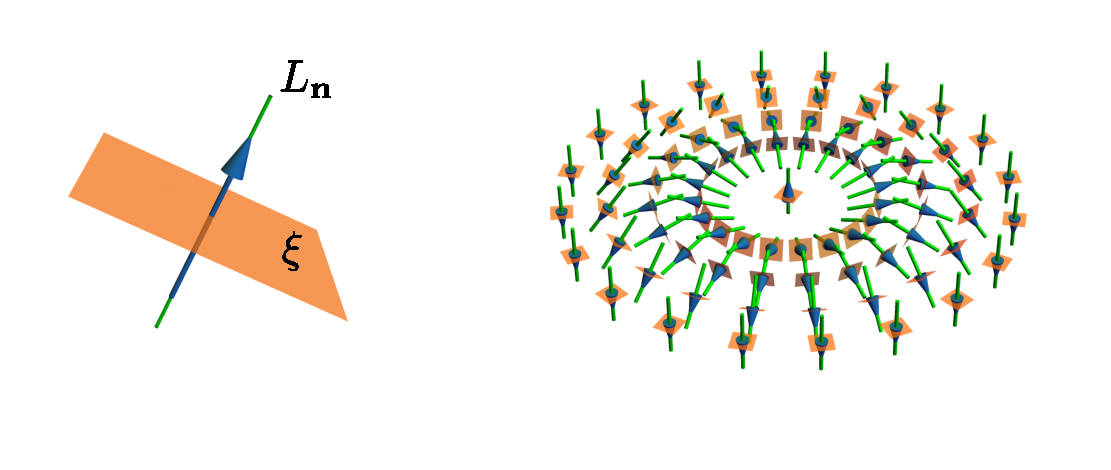
\includegraphics[width=\linewidth]{\IntroductionFigures/SplittingMontage.pdf}
\caption{ The director $\bf n $ splits space into a family of lines $\L$ parallel to it, and a family of planes $\xi$ perpendicular to it: $T \mathbb{R}^3 \approx L \oplus \xi$. Panel (a) shows this splitting at one point, with the director a blue arrow, $L$ the green line and $\xi$ the orange plane. This splitting is shown for an entire Skyrmion texture in panel (b). Compactifying the boundary of this Skyrmion, i.e. considering the outer ring of vectors and planes to really only be one vector and one plane, the Skyrmion texture is topologically the family of normal vectors to $S^2$, and $\xi$ is its tangent bundle. As such, a smoothly varying choice of vectors tangent to the family of planes $\xi$ (section of the bundle) cannot be made (it is worth imagining trying to do so: make some choice of the same fixed vector for all the outer ring of planes, and then try and extend inwards. This amounts to combing one half of the sphere and finding one cannot also comb the other).}
\label{fig:SplittingMontage}
\end{figure}
The terms appearing in~\eqref{eq:FrankFreeEnergy} correspond to the magnitudes of the irreducible components of $\nabla{\bf n}$ under the action of the rotation group $SO(2)$ on $\xi$. These piece together to give a decomposition of $\nabla {\bf n}$ in terms of gradients along $\xi$ and along $L$. Let $E_\bullet$ denote projection onto the subspace $\bullet$, and $\nabla^\bullet \bf n = (\nabla \bf n)|_\bullet$ denote restriction of the linear map $\nabla \bf n$ onto the subspace $\bullet$. Then $\nabla {\bf n}=\nabla^{L}{\bf n}E_L + \nabla^\xi {\bf n}E_\xi$, where 
\begin{align}
    &\nabla^L {\bf n}=  {\bf n}^* \otimes ({\bf n} \cdot \nabla) {\bf n}\label{eq:GradientDecompositionpar}, \\
    &\nabla^\xi {\bf n}= \frac{\nabla \cdot {\bf n}}{2}I_\xi + \frac{{\bf n} \cdot \nabla \times {\bf n}}{2} J + \Delta .
    \label{eq:GradientDecompositionperp}
\end{align}
Here $I_\xi$ is the identity transformation on $\xi$ and $J= \bf n \times \bullet$ is rotation about $\bf n$\footnote{That the splay term appears squared in~\eqref{eq:FrankFreeEnergy} is because the decomposition~\eqref{eq:GradientDecompositionpar},\eqref{eq:GradientDecompositionperp} is for vector order, not nematic order. The additional symmetry $\bf n \sim -n$ forces us to square this term. That the twist term is squared is because nematics are achiral. In a cholesteric liquid crystal \citep{Bellar2014} one has $({\bf n} \cdot \nabla \times {\bf n}+q_0)^2$, giving a linear term on expansion of the square.}. The geometry of $\nabla^\xi \bf n$, and $\Delta$ in particular, has been explored in Ref. \citep{Machon2016b}. $\nabla^\xi \bf n$ describes how $\bf n$ varies as one moves in directions lying in the orthogonal plane $\xi$; when $\bf n$ is the normal to a surface, -$\nabla^\xi \bf n$ is a classical object in the differential geometry of surfaces called the shape operator. The decomposition~\eqref{eq:GradientDecompositionperp} corresponds to its breakdown into an isotropic piece $I_\xi$, an antisymmetric piece $J$ and a traceless symmetric piece $\Delta$. When $\bf n$ is the normal to a surface the antisymmetric piece $J$ vanishes, and $\Delta$ is just $\nabla^\xi \bf n$ with the isotropic part removed --- the eigenvectors of $\Delta$ then coincide with those of $\nabla^\xi \bf n$ and pick out the two directions of principal curvature in $\xi$. This interpretation extends to the general case where $J \neq 0$, and the eigenvectors of $\nabla^\xi \bf n$ do not necessarily exist, motivating the name ``biaxial splay'' for its mode of distortion. The geometry of $\nabla^L \bf n$ is less well explored. It describes the bending of the director field: if one traces a single curve to which $\bf n$ is tangent, then $\nabla^L \bf n $ gives the classical curvature from the differential geometry of space curves \citep{DoCarmoBook}. A more complete account of its geometry and topology will be the topic \S\ref{ch:TwistBend}.
 
Each of the pieces in~\eqref{eq:GradientDecompositionpar}, \eqref{eq:GradientDecompositionperp} is manifestly geometric, but they also represent topological information as canonical sections of vector bundles defined by the director. The families of lines $L$ and planes $\xi$ vary smoothly with the director, and such smoothly varying families of vector spaces are called vector bundles \citep{TuBook,MilnorStasheffBook}. The most famous example of a vector bundle, and the interesting properties they can have, is the family of planes tangent to $S^2$ called its tangent bundle $T S^2$. A smoothly varying choice of vector in each of these tangent planes is called a section of the tangent bundle (or more commonly simply a vector field), with the set of all sections denoted $\Gamma (TS^2)$. Famously, the Poincar\'e-Hopf theorem tells us one cannot `comb a sphere' \citep{Milnor1997}, in other words one cannot find an everywhere nonzero section of the tangent bundle to the sphere. This failure is connected to the topology of $S^2$; if one sums the windings of all the zeros in any section one obtains the Euler characteristic of $S^2$. An entirely analogous result holds for any vector bundle; the zeros of a section of a vector bundle encode its Euler class \citep{BottTuBook, MilnorStasheffBook}. Returning to~\eqref{eq:GradientDecompositionpar}, \eqref{eq:GradientDecompositionperp}, $\nabla^\xi \bf n $ is a section of the bundle $\xi^* \otimes \xi$ --- it maps vectors orthogonal to $\bf n$ into vectors orthogonal to $\bf n$ --- and the bend $\nabla^L {\bf n} \in \Gamma (L^* \otimes \xi)$. Both probe the topology of $\xi$ and, loosely speaking, as $\xi$ is in one-to-one correspondence with the director $\bf n$ this topology carries over to $\bf n$. The zeros of $\Delta$, called umbilic lines in analogy to the umbilic points of the differential geometry of surfaces, have been investigated in Ref.~\citep{Machon2016b}. The zeros of $\nabla^L \bf n$, which we will call $\beta$ lines, will be the subject of \S\ref{ch:TwistBend}.

The umbilic and $\beta$ lines are natural geometric structures found in any vector field. However, they assume a particular relevance when strongly coupled to the energetics of the liquid crystal texture. One way to do this is to frustrate the liquid crystal with boundary conditions, as in the disclinations of figure~\ref{fig:KnottedLiquidCrystal}. Another is to pass to a different phase of liquid crystal, where such coupling exists. In the case of umbilic lines, this setting is the cholesteric phase \citep{Bellar2014}, in which the liquid crystal has a preference for nonzero twist; $\Delta$ turns out to be related to the axis of this twisting~\citep{MachonThesis, AlexanderBook}, and its zeros thus encode energetic frustration inside the cholesteric~\citep{Machon2016b}. For $\beta$ lines, the natural setting is a recently discovered phase of liquid crystal, the twist-bend or splay-bend nematic \citep{Cestari2011,Chen2013,Borshch2013,Lavrentovich2018}. These materials, comprised of banana shaped molecules, have an energetic preference for everywhere nonzero bend. A second focus of \S\ref{ch:TwistBend} will be on this interplay between geometry and energetics in twist-bend nematics. 

\section{Modern knotted fields: excitable media}
\label{sec:FN}

\setlength{\epigraphwidth}{5in} 
\epigraph{``In excitable media we may have a new context in which something like a vortex atom theory can live again, strangely transfigured.''}{A. T. Winfree, The Geometry of Biological Time, Chapter 9.}
\begin{figure}[htbp]
\centering
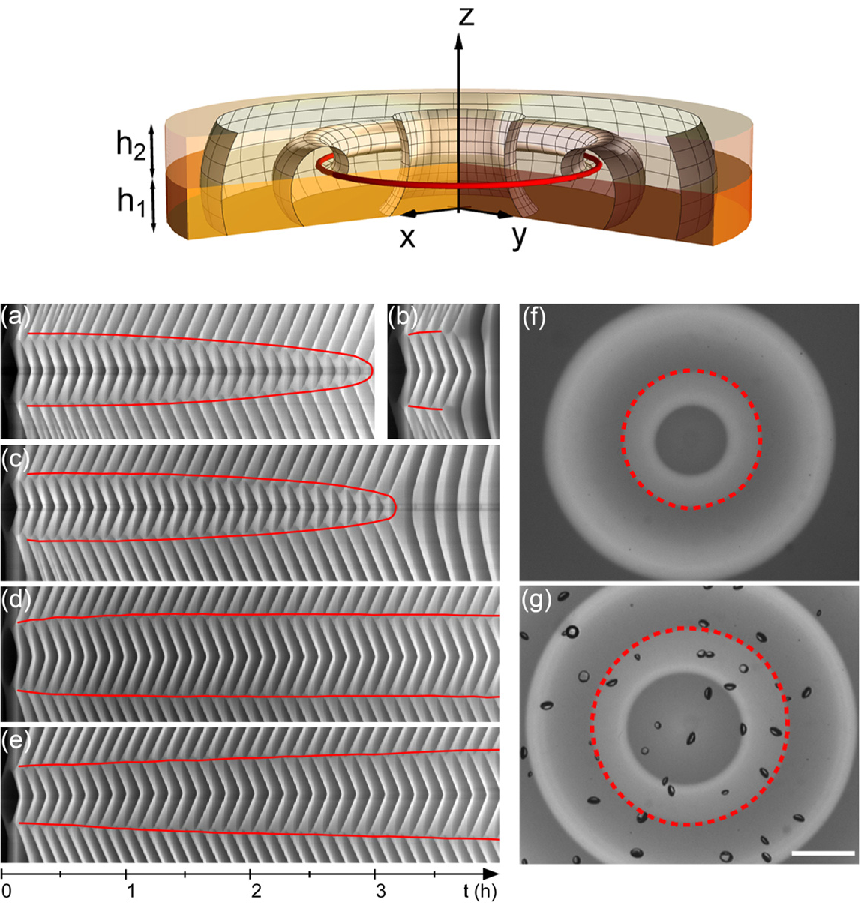
\includegraphics[width=\linewidth]{\IntroductionFigures/FNExperimental.pdf}
\caption{Top Panel: Schematic illustration of a vortex ring in excitable media. A dish of the Belousov-Zhabotinsky reagent supports an axially symmetric spiralling wave of chemical activity (meshed wavefronts) emanating from a ring shaped singularity shown in red. Bottom Panel: An experiment realising this setup. (a)--(e) shows a time series of the dish viewed side on, i.e the $x$-$z$ plane, over $4$ hours. The rotation period of the wave itself is $390$s $\approx 6$--$ 7 $ mins. In each frame, the ring appears as a pair of points with wavefronts emanating from it, which collide in the middle of the dish. Over time the ring moves, tracing the curves shown. Depending on the heights $h_1$ and $h_2$ it may shrink (a), (c), reach a steady radius (d) or expand (e). (f) and (g) show the ring from above ($x$-$y$ plane) over $3$ hours. Setting spatial scale, the white bar in (g) corresponds to $5$ mm. Figures reproduced from Ref.~\citep{Totz2015}.}
\label{fig:FNExperimental}
\end{figure}

We now come to our final example of knotted fields, those found in excitable media. We might have discussed them immediately after fluids and superfluids, and indeed we will see closer similarities to those systems than to liquid crystals. That we chose not to is a reflection of their relative lack of experimental development. By way of prelude, the modern state of affairs in these systems is that the analogy to a fluid vortex ring can be generated experimentally \citep{Steinbock2006,Azhand2014, Totz2015}. Figure~\ref{fig:FNExperimental} shows a schematic of a thick dish of the Belousov-Zhabotinsky (BZ) reagent, a medium which supports waves of propagating chemical activity. Axially symmetric waves of such activity spiral outwards from a `singular' ring shown in red --- exactly what is occurring on this ring will be discussed below. Beneath it is an experimental realisation of this setup from Ref.~\citep{Totz2015}, viewed from the side in figures~\ref{fig:FNExperimental}(a)--(e) and from the top in figures~\ref{fig:FNExperimental}(f)--(g). From the side the ring appears as a discontinuity in the emitted wavefronts, with a second such discontinuity where the fronts collide in the middle of the dish. Figures~\ref{fig:FNExperimental}(a)--(e) show stacks of snapshots of different rings evolving over time, with the overlaid red curves tracking their position. They show, firstly, that the rings stably persist over several hours, and secondly that they have their own dynamics, expanding, contracting or reaching a stable radius (the outcome may be experimentally tuned). The topological possibilities, dynamics, and organisation of the entire excitable medium by these rings are the subject of this section, and of \S \ref{ch:FitzHughNagumo}. These rings have not yet been experimentally tied in nontrivial configurations --- as we shall see in this section, such an experiment would be extremely interesting.

\subsubsection{Excitable media}

The building block of an excitable medium is an excitable oscillator, something which rests in a quiescent locally stable state but which, given a small kick, becomes excited before relaxing back to quiescence. A prototypical example is a nerve cell. Given an electrical input, the cell `fires', becoming excited, before slowly relaxing back to its resting state where it can be triggered again. An excitable medium is a continuum of these oscillators, all coupled together, in our case by diffusion of activity from one oscillator to its spatial neighbours. Such media support waves of activity, where an excitation in one oscillator triggers its neighbours to `fire' also. A pleasing example of such waves is a grass fire \citep{Winfree1983}. The oscillators are blades of grass. Their resting state is unburnt, their excited state burnt. After burning, the blades slowly grow back, able to be burnt again. A field of grass, the excitable medium, supports a wave of excitation, i.e. a moving front of grass fire. Note the front has a leading edge (the transition from unexcited to excited) and a trailing edge (the transition from excited to unexcited).

There is an enormous experimental and theoretical literature on systems exhibiting this sort of behaviour; for references see \citep{WinfreeBook}. We present a minimal mathematical model, which shall be the focus of \S\ref{ch:FitzHughNagumo}, and which provides an effective description of many more complex excitable media \citep{WinfreeBook}: the FitzHugh-Nagumo model \citep{FitzHugh1961,Nagumo1962}
\begin{equation}
\label{eq:FN}
\frac{\partial u}{ \partial t} = \frac{1}{\epsilon}\biggl(u - \frac{1}{3}u^3 -v\biggr) + \nabla^{2} u,\hspace{2em}    \frac{\partial v}{ \partial t} = {\epsilon}(u + \beta -\gamma v) ,
\label{eq:FN}
\end{equation}
Here $u(\bf {x} ,t)$ , $v({\bf x},t)$ are two real valued scalar fields, with $\epsilon,\gamma,\beta$ model parameters. The coupling which turns this system from an excitable oscillator to an excitable medium is through diffusion $\nabla^2 u$, in this instance in the $u$ variable only (although variants with diffusion in each variable also exist). The phase plane for the differential equation system without diffusion is shown in figure~\ref{fig:FN}(a), with parameter choices which will generate an excitable oscillator. The system has a fixed point $(u^*,v^*)$ (black dot), but given a finite perturbation in $u$ it will execute a large loop in phase space called the excitation-recovery loop, jumping to the upper branch of the $u$ nullcline, crawling along it until the first inflection, whereupon it jumps to the lower branch and crawls again back to the fixed point (black arrows in the figure). In the sense that a perturbation in $u$ instigates this loop, $u$ might be considered an `excitor' variable and $v$ a `recovery' variable.
\begin{figure}[htbp]
\centering
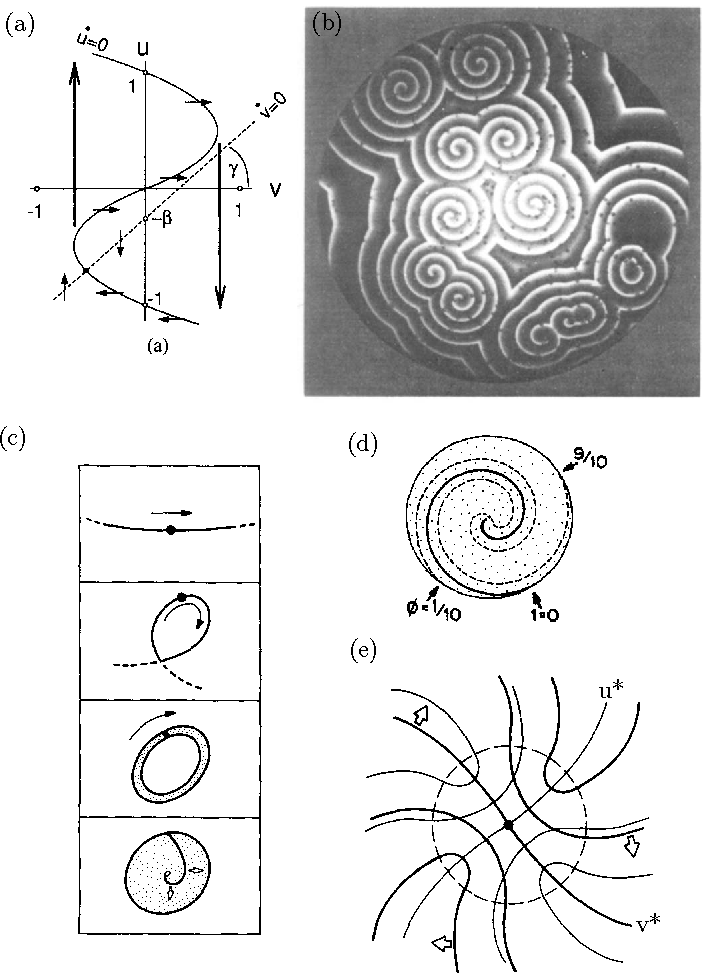
\includegraphics[width=0.8\linewidth]{\IntroductionFigures/FN.pdf}
\caption{Spiral waves in two dimensions. (a) The phase plane of the FitzHugh-Nagumo model~\eqref{eq:FN}, with $u$ and $v$ nullclines (solid and dotted curves), fixed point (black dot) and excitation-recovery loop (large black arrows) shown. This loop is topologically a circle $S^1$, and progression through a cycle of excitation-recovery can be described by a phase $\phi \in S^1$. (b) Spiral waves in a dish of the BZ reagent. (c) --(e) The anatomy of a single spiral wave. In (c) one imagines setting a pulse of excitation running around a closed loop, which gradually thickens until the propagation time around its inner edge is faster than the medium can recover from. The resulting structure is a spiral wave. (d) shows its phase description, with three example isophase spirals shown. (e) A qualitative picture of the $(u,v)$ field around a spiral wave vortex. Away from the vortex the contours are parallel, but inside they necessarily cross one another transversally. Figures reproduced from Ref.~\citep{Winfree1983}. }
\label{fig:FN}
\end{figure}

\subsubsection{The topological possibilities of excitable media}

The key topological observation is that the excitation-recovery loop is a circle $S^1$. In a portion of excitable media $M$, the state of a typical point lies somewhere on this loop, and thus we can describe the system with a map $\phi : M \rightarrow S^1$, a situation encountered before in superfluids. Concretely mapping between $(u,v)$ and $\phi$ may be achieved via something of the form $(u,v) = (2 \cos \phi - u^*, \sin \phi - v^*)$, stretching $S^1$ over the excitation-recovery loop. That the system is characterised by the phase field $\phi \in S^1$ immediately implies the potential existence of knotted and linked vortices if our domain $M$ is three-dimensional, again by simple analogy with superfluids. What makes this system so interesting is that the character and dynamics of these phase singularities are very different to what we have encountered before. 

In two dimensions these singularities are at the core of spiral waves, a collection of which are shown in the BZ reagent in figure~\ref{fig:FN}(b). The anatomy of a single spiral wave is dissected in figure~\ref{fig:FN}(c)--(e). In figure~\ref{fig:FN}(c), one imagines taking an initially thin ring of excitable medium and setting a wave of excitation running around it. If the ring is thickened, we expect some spatial variation in the wavefront--- it turns out that given isotropic diffusion in~\eqref{eq:FN} it takes the shape of an involute spiral started from the inner edge of the ring \citep{WinfreeBook}. This thickening process happily continues until the time taken for the inner edge of the wave to circulate once is comparable to the recovery time of the medium, a condition which defines a `core region', inside of which the $(u,v)$ states of points leave the excitation-recovery loop and so cannot be reliably assigned a phase $\phi$ (this is analogous to what happens inside the healing lengthscale which sets vortex core size in superfluids). A phase description in which the core is idealised to zero radius is shown in figure~\ref{fig:FN}(d), and a qualitative picture of the corresponding contours of $(u,v)$ is shown in figure~\ref{fig:FN}(e). These `rotors' periodically emanate waves of excitation which organise the entire medium, splitting it into domains separated by shock structures where two wavefronts coincide and annihilate (figure~\ref{fig:FN}(b)).
\begin{figure}[htbp]
\centering
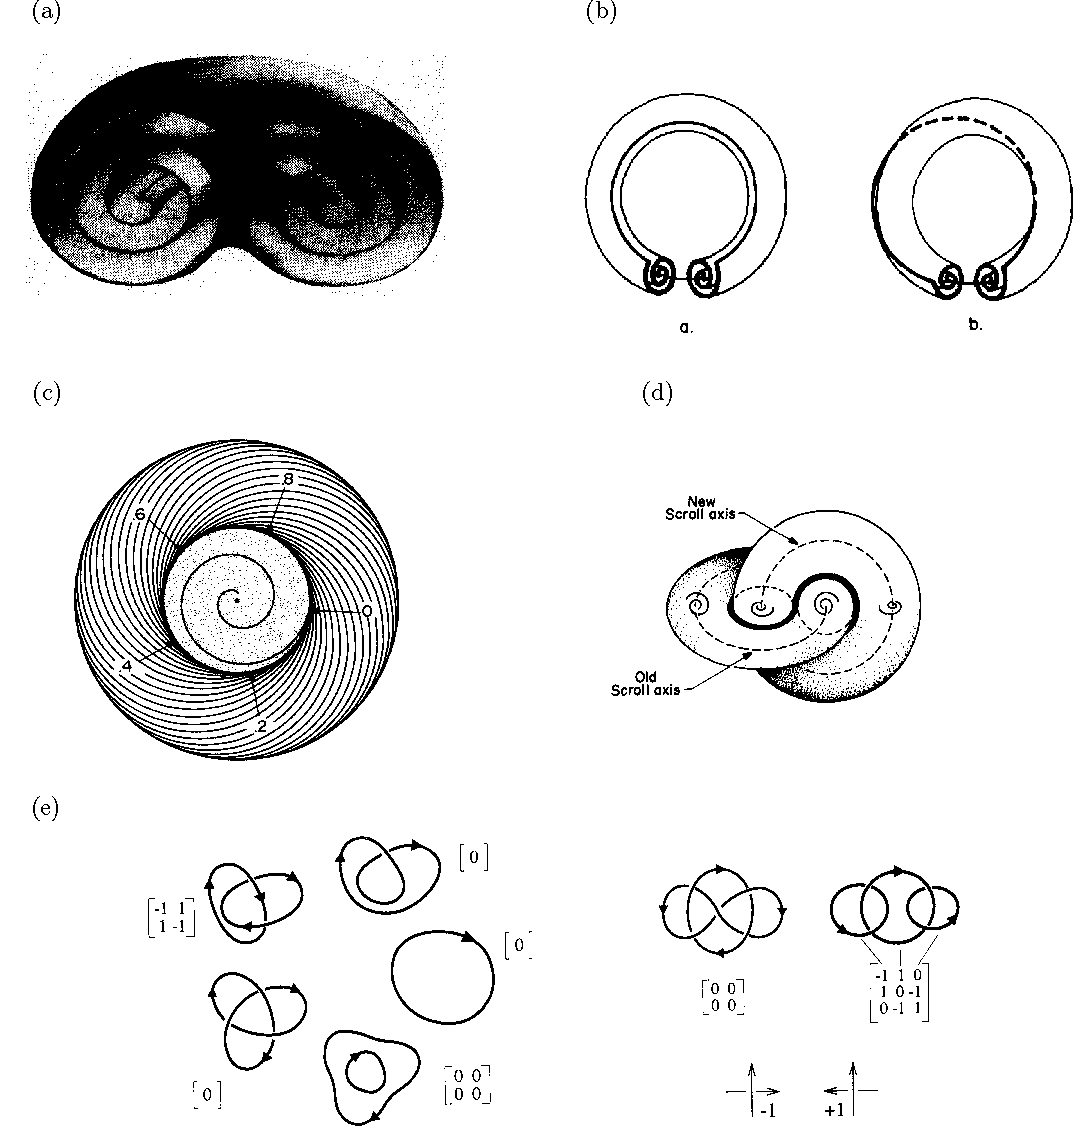
\includegraphics[width=\linewidth]{\IntroductionFigures/FN3D.pdf}
\caption{The topological possibilities of knotted vortices in excitable media. (a) A spiral wave rotated around an axis of symmetry forms a scroll wave, shown in cross section with wavefronts in grey. This is the system realised in figure~\ref{fig:FNExperimental}. (b) Cutting a scroll wave, putting a full turn of each phase contour into it, then gluing back together. (c,d) This twisted scroll ring has a full cycle of phase around its equator (points $0$ through $8$ in panel (c)), necessitating the existence of a second twisted scroll ring linking the first, shown in (d). (e) Two groups of knotted vortices, with transmutations topologically allowed between neighbouring elements of each group. The matrices shown have $(i,j)$th element $Lk(C_i,C_j)$, where $Lk(C_i,C_i):= SL(C_i)$. Note each row (and column) sums to zero, an expression of~\eqref{eq:SelectionRule}. Figures reproduced from Refs.~\citep{Winfree1983, Winfree1983b, Winfree1990}.}
\label{fig:FN3D}
\end{figure}

In three dimensions, we have a linelike phase singularity, a vortex filament, emitting `scroll waves'. The geometric and topological possibilities of linked and knotted vortex filaments were first investigated in a series of papers by A.T. Winfree and S. Strogatz \citep{Winfree1983, Winfree1983b, Winfree1983c, Winfree1984}. The simplest possibility is for the filament to close into a ring, emitting axially symmetric waves which fill space as shown in figure~\ref{fig:FN3D}(a). This is the situation encountered experimentally in figure~\ref{fig:FNExperimental}. However, Winfree and Strogatz demonstrated numerous other possibilities. For example, we once again have internal structure along the singularity, in this case the angle the $\phi=0$ contour (say) makes with the filament in successive cross sections along it, which opens up the possibility of self-linking. The simplest such scenario, a twisted scroll wave, is shown in figures~\ref{fig:FN3D}(b)--(c). Focusing on figure~\ref{fig:FN3D}(c), we note that such twisting implies a full cycle of phase about a line threading the hole in the ring. In other words, a second phase singularity must exist along this line too! Closing this line into a second loop, we obtain figure~\ref{fig:FN3D}(d); two scroll rings, each with linking and self-linking number (+)1. Winfree and Strogatz extend this line of reasoning in a manner similar to that of Moffatt in Ref.~\citep{Moffatt1969} to derive a topological selection rule on allowed configurations of knotted vortices: 
\begin{equation}
    0 = \sum_{i,j, i\neq j} Lk(C_i,C_j) + SL(C_i), \quad \forall i. 
    \label{eq:SelectionRule}
\end{equation}
This rule has a similar feel to the helicity count of~\eqref{eq:HelicityCount}, but its content is slightly different. It is a condition each knotted loop in a link must satisfy in order for the whole to exist. In fact a separate continuum definition of a helicity has been given \citep{Trueba2009} but it is currently not clear (to me at least) how the concepts interlink; it is an interesting question for further study \footnote{~\eqref{eq:SelectionRule} corresponds to giving the link its Seifert framing~\citep{Winfree1983c,MoffattBook}, already seen in superfluids in footnote~\ref{footnote:Seifert}, for which $\mathcal{H}=0$.}.

\subsubsection{The dynamical possibilities of excitable media}

Provided the topological constraint~\eqref{eq:SelectionRule} remains satisfied, there is no reason link reconnections cannot occur, as they do in the other systems we have discussed. In figure~\ref{fig:FN3D}(e) we show two groups of allowed knotted vortices, and within each group transmutations are topologically allowed. As Winfree and Strogatz note, questions of whether or not they actually occur in a given excitable medium ``probably depend sensitively on the exact kinetics of the medium'' \citep{Winfree1984}. In the experiment of figure~\ref{fig:FNExperimental}~\citep{Totz2015} we saw that these vortex lines are not merely static emitters of wavefronts, they have their own dynamics, and one has no \emph{a priori} reason to expect these dynamics to preserve topology. What is absolutely remarkable is that, in a certain parameter regime in the FitzHugh-Nagumo model, it was found that they do \citep{Winfree1990,Henze1993}. Using $\epsilon = 0.3, \beta = 0.7, \gamma=0.5$, a stable vortex ring was found in \citep{Courtemanche1990}, shown in figure~\ref{fig:FNKnots}(a), followed by a stable trefoil knot \citep{Henze1991}(in a slightly different kinetics) and then a variety of apparently stable knots and links \citep{Henze1993} summarised in figure~\ref{fig:FNKnots}(b). An account of this first period of development may be found in Refs.~\citep{Winfree1990, WinfreeBook,WinfreeChapter}. Subsequent work \citep{Sutcliffe2003} confirmed a wide basin of stability for the trefoil knot and the Hopf link over substantially larger time periods than the original trefoil simulations were run for. More recently, Maucher and Sutcliffe \citep{Maucher2016} showed that the FitzHugh-Nagumo dynamics is even capable of simplifying a tangled unknot into a unique canonical round form, as well as demonstrating stable forms for more complex knots --- the figure-eight and torus links in certain geometries \citep{Maucher2017}. A simplification of an unknot with 13 crossings in projection is shown in figure~\ref{fig:FNKnots}(c), with a cross section to show the associated wavefield in figure~\ref{fig:FNKnots}(d) (one might compare to figure~\ref{fig:FN}(b)). The stable torus and figure-eight knots with associated minimal lengths are shown in figure~\ref{fig:FNKnots}(e).
\begin{figure}[htbp]
\centering
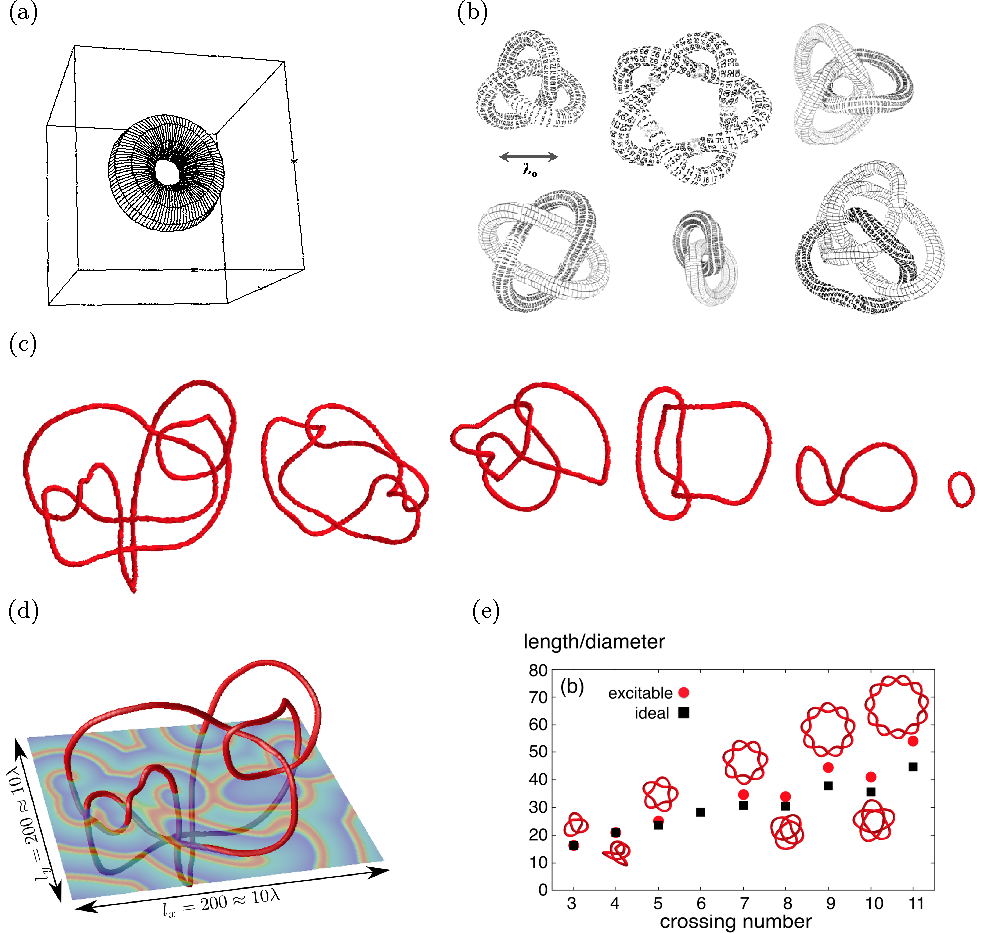
\includegraphics[width=\linewidth]{\IntroductionFigures/FNKnots.pdf}
\caption{Stable knotted vortices in the FitzHugh-Nagumo model. (a) A vortex ring contracts to a stable radius and drifts at constant velocity; its radius is 0.23$\lambda_0$, where $\lambda_0$ is the wavelength of the spiral wave in the medium (see scale bar in panel (b)) . (b) An assortment of apparently stable knotted and linked vortices found in Ref.~\citep{Henze1993}. The tube around the knots is of diameter $\lambda_0/\pi$. The stability of the trefoil knot and Hopf link were subsequently confirmed in Ref.~\citep{Sutcliffe2003} (the others are, in fact, unstable in the bulk). (c,d) The FitzHugh-Nagumo dynamics are capable of simplifying a tangled, but unknotted, curve to the canonical round form of panel (a); panel (c) shows an example simplification, with a cross section through the vortex knot in panel (d) showing the wavefield.(e) Recently, stable forms for torus knots and the figure-eight knot were found. Their geometries are shown here, alongside their lengths as compared to ideal ropelengths. Figures reproduced from Ref.~\citep{Winfree1990,WinfreeChapter,Maucher2016,Maucher2017}.}
\label{fig:FNKnots}
\end{figure}
These numerical findings are in stark contrast to what we saw in fluids, superfluids and liquid crystals (indeed, in most knotted fields), and invite a series of questions: What determines the dynamics of these vortices? How are reconnections avoided? What is the mechanism of knot untangling? Are all knots stable, and if so can we predict their shapes? In some form these questions have existed since the first knotted vortices were discovered. Initial theoretical work focused heavily on the idea that their laws of motion could be explained by a `local geometry hypothesis'~\citep{Keener1988,Keener1992,Biktashev1994,Henry2002,Echebarria2006,Dierckx2010} in which dynamics at each point on the curve were governed by some local law of motion involving its curvature, the twist of spiral wave phase etc. After a perturbative theory for such a law was developed~\citep{Keener1988,Keener1992, Biktashev1994}, substantial work went into testing whether or not this was the case~\citep{Winfree1990,Henze1993}, of which an account may be found in \citep{WinfreeChapter}. Summarising very coarsely, such laws found some success in describing isolated filaments, but of course encounter problems whenever interfilament interactions are required. The problem is that evidence ultimately suggested such interactions were integral to describing stable knots \citep{Henze1993,WinfreeChapter}, and as such a local geometry hypothesis failed to account for their dynamics. The observed untangling without reconnection of unknots shown in figure~\ref{fig:FNKnots}(e) \citep{Maucher2016} further casts doubt on whether such a law could be made to work. 

We remark that the idea of reducing the dynamics of an entire field to that of a curve is not unique to excitable media, but cuts across knotted fields. In particular the idea is similar to the Local Induction Approximation (LIA) in fluids and superfluids \citep{Saffman1992}, in which the Biot-Savart law of motion governing vortex lines is approximated by a dominant contribution arising from local curvature, which leads to motion binormal to the curve --- in the case of a vortex ring, drift perpendicular to the plane it lies in, a feature shared by the rings studied here \citep{Winfree1990}. Further, exact knotted solutions to the LIA \emph{do} exist \citep{Hasimoto1972,Kida1981}, and one might have hoped something similar applied here. Note however that the LIA breaks down in fluids too, and further that the nature of the fields surrounding the vortices is quite different between the two cases. One crucial difference, as we shall see, is that in excitable media waves propagate without attenuation for potentially arbitrary distances, making a theoretical decoupling of distant segments of the knot difficult. 

In summary, the questions posed above are not satisfactorily answered. Our attempts to explore them, with a focus on systematically testing knots for stability and exploring the importance of nonlocal filament interactions, form \S \ref{ch:FitzHughNagumo}. The potential for experimentally accessible, and spontaneously stable, knotted fields is a major motivator for this work.

\section{This thesis}

This thesis is primarily about knotted fields in soft matter systems, systems that may be loosely characterised as those in which geometry plays a fundamental role, and which may undergo substantial deformations in response to external forces, changes in temperature etc. All three of the systems described above might be considered examples of soft matter systems. One might ask ``why choose soft matter?'' and we hope that our descriptions of the experimental possibilities of such systems provide an immediate answer. Their combination of rich geometric structure and experimental accessibility make them natural testbeds for exploring knotted fields in all their guises. In our focus on soft matter we have of course been selective, completely neglecting discussion of theoretical and computational advances in optics \citep{Bode2017,Dennis2017}, electromagnetism \citep{Ranada1989, Ranada1990, Ranada1992,Irvine2010,Kedia2013,Kedia2016,Arrayas2017,Kedia2018} and high energy physics \citep{Faddeev1997, Houghton1998,Battye1998,Battye1999, Sutcliffe2007}. Even within the realm of soft matter we have been selective; fluids stand out as the first and most highly developed examples of knotted fields, and as such it was natural to discuss them. Beyond that, as well as important examples of knotted fields in their own right, our presentation of material on liquid crystals and excitable media serve as background and motivation for the research topics addressed in this thesis.

As for the research topics themselves, they fall under the broad heading of `investigations into knotted fields in soft matter', but each is a distinct story. Primarily they were chosen simply in response to current interesting questions in knotted fields. As for \S\ref{ch:FitzHughNagumo}, Maucher and Sutcliffe's paper on unknot simplification \citep{Maucher2016} was published in 2016, and one might take it as marking renewed interest in questions around the FitzHugh-Nagumo model --- there is a gap of $13$ years between it and the last publication on the matter \citep{Sutcliffe2003}. Coupled with improved computational abilities\footnote{Compare the description in Ref.~\citep{Henze1993} of running code on a CRAY supercomputer to my own experience on my laptop and the Warwick cluster.}, new ideas about knot initialisation, and the recent experiments we discussed in \S \ref{sec:FN}, it seems a natural time for new investigation. \S\ref{ch:TwistBend} is again a development of recent questions about the geometry and topology of liquid crystal gradients; our focus will be on the topology of bend distortions. As we have seen, more theoretical attention has been paid to orthogonal gradients and twist \citep{Bellar2014,Machon2016, Machon2017} than to bend (however there is recent work on splay and bend in two dimensions \citep{Niv2018}) and it is natural to try and complete the picture. The recent discovery of twist-bend and splay-bend nematic phases, of which the first review was published in 2018 \citep{Lavrentovich2018}, provides further motivation as a natural experimental setting for theoretical constructs, a role the cholesteric plays for twist. The content of \S \ref{ch:Maxwell}, on theoretical constructions for initialising knotted vortices, is a little different: it initially arose out of a practical need to do just that in \S\ref{ch:FitzHughNagumo}. Many other methods exist and will be discussed in \S\ref{ch:Maxwell}, but in one way or another they did not suit our needs, either because the geometries of knot they allowed were restricted, or they were computationally problematic. In attempting to solve this practical problem, we were led to re-evaluate Maxwell's work on the solid angle function \citep{Maxwell2}, extending it to knots and discovering connections between the various different methods he proposes for constructing the function, as well as connections to modern work on curve framings, writhe etc. As a result, this chapter has a `half theoretical, half practical' feel. Its content was subsequently used in the simulations presented in \S\ref{ch:FitzHughNagumo} and in constructing the self-linkings of bend zeros described in \S\ref{ch:TwistBend}.

We now provide a more technical summary of the content of each chapter, with reference to the foregoing discussion.

\subsubsection{\S \ref{ch:Maxwell}: Maxwell's Theory of Solid Angle and the Construction of Knotted Fields}

This chapter addresses a question which cuts across particular systems, and has not been much discussed above: Theoretically, how should one construct a knotted field? In order to simulate a knotted superfluid vortex (figure~\ref{fig:SuperFluidMontage}), a knotted vortex in the FitzHugh-Nagumo model (figure~\ref{fig:FNKnots}), or any other knotted system one needs a method of initialising a topologically correct configuration before running dynamics. For the above examples, this amounts to constructing a phase field $\phi \in S^1$ containing a phase singularity with the topology (and possibly geometry) of the desired knot. 

In this chapter we propose the solid angle function of a link $K$, defined by Maxwell in his \emph{A Treatise on Electricity and Magnetism} \citep{Maxwell2}, as a natural solution to this problem. We provide a systematic description of this function as a means of constructing a knotted field for any curve or link in $\mathbb{R}^3$. This is a purely geometric construction in which all of the properties of the entire knotted field derive from the geometry of the curve, and from projective and spherical geometry. We emphasise a fundamental homotopy formula as unifying different formulae for computing the solid angle. The solid angle induces a natural framing of the curve, which we show is related to its writhe $Wr$ and use to characterise the local structure in a neighbourhood of the knot. Finally, we discuss computational implementation of the formulae derived, and give illustrations for how the solid angle may be used to give explicit constructions of knotted vortices in excitable media and knotted director fields around disclination lines in nematic liquid crystals. Part of the work in this chapter consists of an implementation of the methods described in C++: it may be found at \href{https://github.com/garethalexander/SolidAngle}{https://github.com/garethalexander/SolidAngle}.

TODO:INCLUDE IN THE APPENDIX

\subsubsection{\S \ref{ch:TwistBend}: Bend Geometry in Liquid Crystals}
TODO: FILL THIS IN

\subsubsection{\S \ref{ch:FitzHughNagumo}: Stable and Unstable Vortices in Excitable Media}
In \S \ref{sec:FN} we discussed the discovery of several apparently stable knotted vortices in the FitzHugh-Nagumo model, as well as the dynamics' remarkable ability to simplify unknots without reconnections. We also saw that the mechanisms underlying these phenomena are still ill-understood, and posed the following questions: What determines the dynamics of these vortices? How are reconnections avoided? What is the mechanism of knot untangling? Are all knots stable, and if so can we predict their shapes? This chapter is an exploration of these questions. We perform a systematic survey of the dynamics of all knots with at most eight crossings, establishing that the generic behaviour is of unsteady, irregular dynamics, with prolonged periods of expansion of parts of the vortex. We show that the mechanism for the length expansion is a long-range “wave-slapping” interaction. We also show that there are stable vortex geometries for certain knots; in addition to the unknot, trefoil, and figure-eight knots reported previously, we have found stable examples of the Whitehead link and $6_2$ knot. We give a thorough characterisation of their geometry and steady-state motion. For the unknot, trefoil, and figure-eight knots we greatly expand previous evidence that FitzHugh-Nagumo dynamics untangles initially complex geometries while preserving topology, and discuss the mechanisms at play.






